\documentclass[12pt,twoside]{report}
\usepackage[a4paper,width=150mm,top=25mm,bottom=25mm,headheight=15pt]{geometry}
\usepackage[T1]{fontenc}
\usepackage[utf8]{inputenc}
\usepackage[english,italian]{babel}
\usepackage[export]{adjustbox}
\usepackage{multicol}
\usepackage{graphicx}
% cartella da cui attigere immagini
\graphicspath{ {immagini/} }

% an easier format to achieve as you lose the constraint on equalising page content. 
\raggedbottom

% trasforma i \par in spazi
\usepackage{parskip}

% Commenti multilinea
\usepackage{verbatim}

% Package per le parti di matematica
\usepackage{amsmath}
\usepackage{amssymb}

% Package per inserire il codice
\usepackage{minted}
\usemintedstyle{emacs}
%emacs, manni

% inserire immaggi al top del foglio
\makeatletter
\setlength{\@fptop}{0pt}
\makeatother

% testa e fondo pagina che richiamano il frontespizio durante la lettura 
\usepackage{fancyhdr}
\pagestyle{fancy}

% Nome capitolo in basso a sinistra al posto di \chaptername \thechapter
\renewcommand{\chaptermark}[1]{%
	\markboth{\thechapter.\ #1}{}}
	
% da customizzare a piacere
\fancyhead{}
\fancyhead[RO,LE]{Diagnosis by Numbers}
\fancyfoot{}
\fancyfoot[LE,RO]{\thepage}
\fancyfoot[LO,CE]{\leftmark}
\fancyfoot[CO,RE]{Damiano Gianotti}
% Per cambiare lo spessore delle linee di testa e piè pagina
\renewcommand{\headrulewidth}{0.4pt}
\renewcommand{\footrulewidth}{0.4pt}

% includere i pdf
\usepackage{pdfpages}


% bibliografia
\usepackage[backend=biber]{biblatex}
\addbibresource{references.bib}

\begin{document}
    % !TeX spellcheck = it_IT

\begin{titlepage}
    \pagestyle{empty}
    \begin{center}
        \LARGE{\textsc{Università degli Studi di Torino}}                           \\
        \Large{\textsc{Dipartimento di Informatica}}
        \vskip 10pt
        \Large{\textsc Corso di Laurea in Informatica}                              \\
        \vskip 20pt
        
\includegraphics[width=4cm]{immagini/logo_unito.pdf}                        \\
        \vskip 20pt
        \Large{Tesi di Laurea in Informatica}                                       \\
        \vskip 40pt
        \LARGE{\textbf{Diagnosis by Numbers: }}                                             \\
        \LARGE{\textbf{Uno strumento basato su}}                                   \\
        \LARGE{\textbf{logiche descrittive, "tipicalità" e probabilità}}                                      \\
        \vskip 30pt
        \Large{\textbf{Relatore:}}               \\
        \Large{Prof. Gian Luca Pozzato}          \\
        \vskip 30pt
        \Large{\textbf{Candidato:}}                                                  \\
        \Large{Damiano Gianotti}                                                       \\
        \vskip 40pt
        \textbf{Sessione Ottobre 2019}                                               \\
        a.a 2018/2019
    \end{center}
\end{titlepage}
\thispagestyle{empty}\cleardoublepage
    
	

\thispagestyle{plain}
\begin{center}
	\Large
	\textbf{Diagnosis by Numbers}
	
	\vspace{0.4cm}
	\large
	Uno strumento basato sulle logiche descrittive, "tipicalità" e probabilità
	
	\vspace{0.4cm}
	\textbf{Damiano Gianotti}
	
	\vspace{0.9cm}
	\textbf{Abstract}
\end{center}

Lo stage si pone l’obiettivo di realizzare \textbf{DbN}, un tool di supporto per la \textit{diagnosi differenziale}, 
con applicazione ad un caso di studio in ambito medico, basato su una logica descrittiva con tipicalità e probabilità di avere eccezioni.
La logica in questione consente di generare scenari plausibili ma “sorprendenti”, che consentiranno di formulare
diagnosi non ovvie  (iter alternativi potenzialmente \textit{sorprendenti}) e di stimarne la probabilità. 
Lo strumento potrebbe portare ad ulteriori ricerche, nel caso in cui le spiegazioni
più plausibili non siano quelle corrette e mostrare possibili scenari non banali.
 
Il lavoro iniziale è stato lo studio delle Logiche Descrittive, una famiglia 
di linguaggi formali utilizzati per esprimere (rappresentare) la conoscenza 
in un dominio specifico (detto mondo). Sono quindi alla base dei linguaggi impiegati per lo sviluppo
di ontologie nel Web Semantico, come il Web Ontology Language (OWL).

In seguito, il progetto è partito come estensione della tesi \citetitle{PEAR} \cite{PEAR}. Infatti, dopo averne studiato le caratteristiche importanti, si è cercato di costruire sopra
un diverso sistema di generazione degli scenari e di rafforzarne le componenti di ragionamento, fortemente orientati all'implementazione dell'esempio sei di \citetitle{ProbOfEx} \cite{ProbOfEx}.
Raggiunto questo obiettivo, non banale, si è ottimizzato e pulito il codice
e sono state aggiunte funzionalità aggiuntive, come la creazione di grafici interattivi e costi
diagnostici.

\paragraph{Struttura della tesi} \hfill

Di seguito, il piano di quest'opera.
\begin{itemize}
	\item Il primo capitolo dà una breve infarinatura sulle fondamenta del progetto e descrive schematicamente il lavoro che è stato svolto.
	\item Il secondo capitolo invece fornisce alcune tra le nozioni teoriche più importanti che
	servono per comprendere i meccanismi su cui si basa DbN
	\item Il terzo tratta di quali librerie/linguaggi son state/i utilizzate/i e il perché
	\item Il quarto descrive, in dettaglio, le singole componenti del \textit{software}
	\item Il quinto racconta dei principali problemi presenti e delle possibili idee risolutive
\end{itemize}
	
	\tableofcontents
	
	\chapter{Introduzione}
	\section{Ambiente e metodologie di studio}
%Introduzione alla storia
%delineare il quadro generale

La  ricerca  nel  settore  della  rappresentazione  della  conoscenza  si  concentra da sempre
sulla possibilità di fornire descrizioni ad alto livello di fatti, gerarchie terminologiche
e reti concettuali necessarie ad software ‘intelligenti’, ossia a quelle applicazioni
in grado di ricavare conseguenze implicite (talvolta profonde o nascoste) di conoscenze 
esplicitamente disponibili o facilmente accessibili. \par
In tal senso le Logiche Descrittive si pongono come miglior risposta per questo di problema
poiché riescono a coniugare in modo sapiente l'espressività ed efficienza: 
man mano che gli studi e le sperimentazioni relative alle Logiche Descrittive progrediscono,
le nostre conoscenze e capacità di classificare in modo sottile i vari frammenti dei
linguaggi logici si fanno sempre più profonde ed adeguate alle esigenze dei vari ambiti applicativi.
  
Nel nostro caso, però, si trovano subito delle difficoltà, infatti si presuppone 
la congiunzione di due requisiti contrastanti : il bisogno composizioni sintattiche 
(tipiche dei sistemi logici), e la necessità dell'utilizzo della "tipicalitá".
Uno dei limiti di queste logiche è che non sono in grado di rappresentare proprietà tipiche
e di ragionare sull'eredità rivedibile \cite{ProbOfEx}.
Richiamiamo dunque, in maniera informale, un classico esempio proveniente dalla letteratura: 
immaginiamo di sapere che gli uccelli volano, ma che i pinguini siano uccelli che non volano.
Questa base di conoscenza sarebbe consistente solo se non ci fosse neppure un pinguino. 
Per affrontare questo problema fin dai primi anni '90 sono state approfondite e studiate 
numerose estensioni non monotone delle logiche descrittive.\par
Il programma oggetto delle tesi si basa sulla $\mathcal {ALC}+\mathbf{T}_\mathbf{R}^{ \textsf {P} }\ $. 
Questa, oltre ad avere complessità ExpTime-completa (come la sottostante $\mathcal {ALC}$), combina diverse componenti importanti:
\begin{itemize} \label{itemize: 3 comp}
	\item in primis la logica $\mathcal {ALC}+\mathbf{T}\ $ dove le proprietà tipiche possono 
	direttamente essere descritte dall'operatore $\mathbf{T}$ di “tipicalità“, grazie a cui
 è possibile esprimere che, per ogni concetto $\mathit{C},\mathbf{T}(\mathit{C})$ 
 indica che le istanze di C sono considerate \textit{tipiche} o \textit{normali}.
	Così una $\mathit{TBox}$ potrà contenere inclusioni della forma $\mathbf{T}(\mathit{C})\sqsubseteq \mathit{D}$ 
	a rappresentare che “i tipici $\mathit{C}$ sono anche $\mathit{D}$. A differenza della 
	maggior parte delle altre logiche descrittive questa ci permetterà quindi
	di esprimere e ragionare sulle eccezioni mantenendo una consistenza della base di conoscenza.\cite{DLExtension};
		
	\item il secondo ingrediente necessario sarà una semantica distribuita, simile 
	a quella utilizzata per le logiche descrittive probabilistiche, conosciuta come DISPONTE. 
	L’idea è quindi quella di aggiungere un’etichetta alle inclusioni che indichi la probabilità 
	di tale fenomeno, per poter esprimere quanto sia possibile che un evento eccezionale si verifichi.\par
	Con questa estensione è possibile esprimere fatti del tipo: \par 
	$ \mathbf{T}(\mathit{C})\sqsubseteq_{p} \mathit{D} $ ("abbiamo una probabilità p che un tipico C sia un D") \par 
	direttamente nella base di conoscenza oppure inferire e/o dedurre fatti del tipo 
	\par$ \mathit{p}:\mathbf{T}(\mathit{C})(\mathit{m})$ ("il membro m è un tipico C con una certa probabilità p")\cite{ProbOfEx};
		
	\item il terzo riguarda il rafforzamento della semantica trattato nell'articolo \cite{FromPLtoDL} 
	dove gli autori hanno ristretto la consequenzialità logica ad una classe di
	modelli minimi. L’idea intuitiva è quella di restringere la consequenzialità logica ai
	modelli che minimizzano le istanze atipiche di un concetto. 
	La logica risultante è $ \mathcal {ALC}+\mathbf{T}_\mathbf{R}^{ \mathit{RaCl}}$ la cui semantica vedremo meglio in seguito.
\end{itemize}
Se opportunamente uniti otteniamo proprio $\mathcal {ALC}+\mathbf{T}_\mathbf{R}^{ \textsf {P} }\ $ 
che è caratterizzata dalla \textit{probabilità di eccezionalità} dalla forma:
\[ \mathbf{T}(\mathit{C})\sqsubseteq_{p} \mathit{D} \]
dove $ \mathit{p} \in (0,1) $ il cui significato intuitivo è:
\begin{multline*}
\text{"normalmente, gli elementi } \mathit{C}  \text{ sono } \mathit{D} \\
\text{ e la probabilità di avere elementi } \mathit{C} 
\text{ che non sono } \mathit{D} \text{ è } 1 -\mathit{p}."
\end{multline*}

\section{Motivazioni del lavoro}
Sul fatto che un calcolatore possa trattare i dati statistici e fare predizioni probabilistiche meglio di un essere umano non possono esserci dubbi:
l’essere umano non è tanto portato per il ragionamento statistico, che in genere appare controintuitivo. 
In questo senso DbN potrebbe diventare un aiuto diagnostico prezioso, uno strumento di consultazione del medico, più efficace di trattati e riviste, ma con il grande limite di essere disumanizzante. Infatti il dato rilevante alla diagnosi si raccoglie nel contesto del rapporto medico-paziente e il paziente non racconterebbe a DbN la sua anamnesi come la racconterebbe ad un medico di sua fiducia.\\ 
Va sottolineato che, a causa della logica non standard  utilizzata, DbN non è certo allo stato dell'arte ma, al momento, un semplice ma efficace prototipo.

L’aspetto più interessante è il contesto in cui andrebbe ad inserirsi: in effetti già esistono applicazioni per lo smartphone che dovrebbero aiutare il medico nelle decisioni o, almeno, fornirgli spunti di riflessione e di esercizio. Contrariamente, supportare la diagnostica medica è un problema privo di regole esatte e, in fondo, di ampiezza non limitata che sembra molto al di là delle possibilità di una macchina, ma la presenza di grandi aziende, come \textbf{IMB} con \textbf{Watson}, ci fa chiedere per quanto tempo questo rimarrà così.

L’ultimo aspetto da considerare è relativo ai costi: per ora DbN è un embrione, un piccolo prototipo e non è nemmeno immaginabile cosa costerebbe produrne e renderne disponibile un numero sufficiente a soddisfare tutte le possibili richieste di consulenza. D’altra parte la macchina ha delle potenzialità, e anche da sola può rispondere a diverse richieste, ma sicuramente necessita di ulteriori sviluppi.
Il vantaggio nell'uso di un consulente elettronico risulterebbe molto grande, sia per l’accuratezza delle diagnosi e delle terapie, sia per le implicazioni medico-legali come elemento di buona prassi.

\section{Obiettivi}
Alle luce di queste motivazioni, introduciamo ora i sommi capi del sistema DbN.\\
Presa in esame un'ontologia (o base di conoscenza), più o meno vasta, scritta attraverso le logiche descrittive ed 
arricchita da espressioni di tipicalità e da sintomi/prodromi riguardanti un paziente, l'obiettivo è quello di generare tutte le possibili diagnosi (o spiegazioni), controllarne la veridicità (logicamente parlando) e presentarle in forma grafica, evidenziandone la probabilità e il costo stimato.
Va specificato che, come diagnosi si intende un elenco di scenari, realtà "future" possibili, la cui coerenza con la \textbf{KB} è stata verificata dallo strumento.

I risultati ottenuti e il lavoro svolto troveranno illustrazione in dettaglio nelle successive sezioni.  

%che legame c'è con la logica con tipicalità e probabilità? \\
%cosa fa il sistema, anche solo intuitivamente accennando agli scenari e alla diagnosi.\\




	
	\chapter{Logiche Descrittive}\label{chap: DL}
	% minipremessa
In questo capitolo iniziale forniremo una definizione di \textbf{DL} (Description Logics), analizzeremo le sue componenti e verranno descritte brevemente le sue estensioni più importanti, utilizzate negli ultimi anni.
\section{Informazioni iniziali}
Le logiche descrittive sono una famiglia di formalismi per la rappresentazione
della conoscenza, con la capacità di descrivere ciò che è noto in un dominio di
applicazione (detto mondo). Tale rappresentazione si fonda su strutture importanti,
come grafi o frames, e ha una difficoltà variabile, che dipende dal linguaggio scelto,
poiché l'espressività e la complessità computazionale sono direttamente proporzionali.
Tipicamente i nodi rappresentano concetti (oggetti), che possono
avere proprietà (semplici o articolate) associate. È piuttosto
semplice creare una corrispondenza tra i grafi e le \textbf{DL},
perché queste ultime sono dotate di predicati facilmente equiparabili alle strutture dei grafi:
\textit{predicati} unari corrispondo agli insiemi di individui, 
\textit{predicati} binari rappresentano relazioni tra singoli e infine un meccanismo di istruzioni 
d'inclusione per esprimere proprietà appartenenti ai concetti, come, ad esempio, \textit{Scimmia }$\sqsubseteq$\textit{ Mammifero}.

\begin{figure}[ht]
	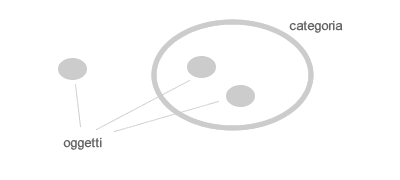
\includegraphics[width=\linewidth]{oggetti-categoria}
	\centering
	\caption{Un esempio di grafo}
\end{figure}

Ecco alcuni esempi riguardanti individui:
\begin{itemize}
	\item \textit{Volpe(foxy)}
	\item \textit{Scappa(foxy)}
	\item \textit{Gallina(coco)}
	\item \textit{Ruba(foxy,coco)}
	\item \textit{Uomo(jhon)}
	\item \textit{Insegue(jhon,foxy)}
\end{itemize}

È anche possibile utilizzare l’intersezione di concetti tramite la sintassi 
\textit{Cane} $\sqcap$ \textit{Taglia Grossa} per cercare individui che 
appartengono ad entrambe le categorie. \\
Ricordiamo che questa tipologia di logiche 
ha alla base quella del prim'ordine, da cui eredita la capacità di 
ragionamento attraverso inferenza, come il \textit{modus ponens}.
Infatti se all'insieme precedente aggiungessimo che:
\[\textit{Mammifero} \sqsubseteq \textit{Animale}\]
allora da questo potremo inferire che $\textit{Volpe}\sqsubseteq\textit{Animale}$.

Per queste e altre caratteristiche peculiari le DL sono ampiamente utilizzate in numerosi
sistemi, proprio per il buon compromesso tra capacità di rappresentazione,
ragionamento e complessità.\\
Vediamo, in breve, alcuni dei principali domini applicativi:

\paragraph{Data mining} 
Questo campo, da sempre al centro di molti dibattiti (anche etici),
ha come scopo "l'estrazione" di dati grezzi. Successivamente, al fine di classificarli,
viene fatto largo utilizzo delle logiche descrittive, per poi,
in seguito, attraverso tecniche di ragionamento, fare inferenza su 
di essi ed ottenere nuova conoscenza.

\paragraph{Medicina}
Fin dagli anni ’80 al centro di molte iniziative è stata la
creazione di una grande ontologia delle conoscenza medica, volta ad essere
di supporto nelle diagnosi. Per far fronte alla scalabilità della base di
conoscenza, si sono spesso utilizzate logiche descrittive basilari.
Rappresenta l'ambito di maggiore interesse per questo studio.

\paragraph{Configuration management}
È uno dei campi di maggior successo: esso include applicazioni che supportano
la progettazione di sistemi complessi grazie  all'unione di componenti multipli.
In particolare attraverso la classificazione di concetti (che possono
anche essere basate su modelli object oriented) si può creare una tassonomia che,
unita alla possibilità di ragionamento, intrinseca nelle logiche
descrittive, permette di trovare con facilità eventuali inconsistenze nel sistema.

\paragraph{Ingegneria del software}
Uno dei primi domini di applicazione: l’idea
alla base era di implementare, attraverso le logiche descrittive, un 
sistema che permettesse allo sviluppatore di trovare facilmente informazioni rilevanti
riguardo ad un sistema particolarmente grande e/o complesso.

\section{Caratteristiche e limiti}
\subsection{Tipologia ed Ingredienti}
% Da rivedere
Ogni logica descrittiva è caratterizzata da una particolare capacità espressiva che
varia a seconda delle possibilità e delle restrizioni imposte nei seguenti elementi:
\begin{itemize}
	\item $\mathcal{AL:}$ indica la logica degli attributi e introduce gli operatori 
	di congiunzione e quantificazione universale ed esistenziale;
	\item $\mathcal{C:}$ descrive la possibilità di usare l’operatore di negazione;
	\item $\mathcal{S:}$ indica la capacità di definire la chiusura transitiva di un ruolo;
	\item $\mathcal{H:}$ fornisce la potenzialità di definire gerarchie tra ruoli;
	\item $\mathcal{O:}$ asserisce la presenza dell'operatore di enumerazione;
	\item $\mathcal{I:}$ permette di riferirsi al ruolo inverso;
	\item $\mathcal{F}\ \mathcal{N}\text{ e }\mathcal{Q:}$ caratterizzano le disponibilità 
	di definire, rispettivamente, la cardinalità funzionale, semplice e qualificata (in ordine di espressività crescente);
	\item $\mathcal{D:}$ descrive la possibilità di riferirsi a domini concreti.
\end{itemize}
\subsection{Monotonicità}
Caratteristica peculiare delle \textbf{DL} nella forma di
\[ KB \models Q \implies KB \cup \{F\} \models Q\]
ovvero, se da una base di conoscenza \textbf{KB} si può concludere un fatto $ Q $, 
allora lo stesso fatto $ Q $ si deduce dalla stessa base di conoscenza arricchita con un nuovo fatto F.

Questa proprietà in sè è molto \textit{importante}, tuttavia non sempre si rivela pratica, anzi, 
esistono contesti (come il nostro) in cui, più che dare benefici, rende difficile il 
ragionamento e la deduzione di nuove informazioni.
Vediamone il perché con un famoso esempio.\\
Consideriamo la seguente base di conoscenza o \textit{Knowledge Base} tratta da \cite{PEAR}:     
\begin{itemize}
	\item[] \textit{Piove} $\implies$ \textit{Prendo(ombrello)}
	\item[] \textit{Piove}
\end{itemize}
si può banalmente concludere che: \textit{Prendo(ombrello)}

Aggiungiamo ora la seguente \textit{formula}
\begin{itemize}
	\item[] \textit{Sono\_Squattrinato}
\end{itemize}
La conclusione precedente rimane lecita anche dopo l'arricchimento della \textbf{KB}.

Aggiungiamo, invece, questa \textit{espressione}
\begin{itemize}
	\item[] \textit{Ho\_Perso(ombrello)}
\end{itemize}
Contro le nostre aspettative/intuizioni la conclusione non cambia, poiché dalle due premesse 
iniziali si giunge allo stessa conclusione senza che la nuova "conoscenza" influisca sul risultato.
Questo semplice modello ci mostra perché è importante, in contesti
specifici, avere dei linguaggi e degli automatismi in grado di tenere conto della 
realtà dei fatti, cioè una logica che possegga una \textbf{eredità rivedibile}.
\section{Il linguaggio base $\mathcal{AL}$}
Un sistema di rappresentazione della conoscenza basato sulle \textbf{DL}
permette di creare, manipolarle e ragionare su diverse \textit{Knowledge Base}.\\
Ma cos'è formalmente una \textbf{KB}?
La base di conoscenza è composta principalmente da una coppia \textit{(T,A)} 
$\mathrm{TBox} \text{ e } \mathrm{ABox}$.
La prima introduce i concetti, insiemi di individui, e ruoli, che
denotano relazioni binarie tra i concetti. \\
Invece per quanto concerne la seconda, essa contiene asserzioni su singoli individui, riguardanti 
concetti della $\mathrm{TBox}$.
Definiamo come descrizioni elementari i concetti e ruoli atomici. Invece trattiamo come 
complesse le descrizioni che possono essere costruite attraverso induzione.
In notazione useremo le lettere $A$ e $B$ per indicare
concetti atomici, la lettera $R$ per rappresentare i ruoli atomici e le lettere $C$ e
$D$ per le descrizioni dei concetti. Qui sotto daremo una definizione di $\mathcal{AL}$ \cite{DLHandbook},
linguaggio minimo di interesse pratico, su cui si basano tutti gli altri linguaggi di questa famiglia.

Le descrizioni di concetti sono definite secondo le seguenti regole sintattiche:
\begin{itemize}
	\item[] \makebox[2cm]{$C,D \to$\hfill}
	\item[] \makebox[2cm]{$\top$ \hfill} (concetto atomico)
	\item[] \makebox[2cm]{$\bot$ \hfill} (top concept - generico)
	\item[] \makebox[2cm]{$\neg\ A$ \hfill} (negazione atomica)
	\item[] \makebox[2cm]{$ C \sqcap D$ \hfill} (intersezione)
	\item[] \makebox[2cm]{$\forall R.C $ \hfill} (restrizione di valore)
	\item[] \makebox[2cm]{$\exists R. \bot$ \hfill} (quantificazione esistenziale limitata)
\end{itemize}
Per definire una semantica formale per i concetti di $\mathcal{AL}$ poniamo alla base 
l'idea di modello e l'idea di funzione d'interpretazione:
\begin{equation} \label{model}
\mathcal{M} = \langle \Delta;fx \rangle
\end{equation} 
\begin{equation} \label{fun}
fx: A \to \Delta
\end{equation}
Definito che le interpretazioni $\mathcal{I}$ sono sottoinsiemi non vuoti di $\Delta$ (dominio dell'interpretazione),
lo scopo di \ref{model} è quello di fornire un significato alle formule, mentre, 
per quanto riguarda \ref{fun}, quello di
permettere di assegnare a ogni concetto atomico $\mathit{A}$ un insieme 
$\mathit{A^{\mathcal{I}} \subseteq \Delta^{\mathcal{I}}}$ 
e per ogni ruolo atomico $\mathit{R}$ una relazione binaria 
$\mathit{R^{\mathcal{I}} \subseteq \Delta^{\mathcal{I}} \times \Delta^{\mathcal{I}}}$.\\
La funzione di interpretazione è estesa alla descrizione di concetti attraverso le seguenti definizioni induttive :
\begin{itemize}
	\item[] \makebox[2cm]{$\top^{\mathcal{I}}$\hfill} = $\Delta^{\mathcal{I}}$  
	\item[] \makebox[2cm]{$(\neg A)^{\mathcal{I}}$ \hfill} = 
	$\Delta^{\mathcal{I}}\backslash A^{\mathcal{I}}$
	\item[] \makebox[2cm]{$(C \sqcap D)^{\mathcal{I}} $ \hfill} = 
	$ C^{\mathcal{I}} \sqcap D^{\mathcal{I}} $  
	\item[] \makebox[2cm]{$(\forall R.C)^{\mathcal{I}}$ \hfill} = 
	$\{x \in \Delta| \forall y.(x,y) \in R^{\mathcal{I}} \to y \in C^{\mathcal{I}} \}$
	\item[] \makebox[2cm]{$(\exists R.\top)^{\mathcal{I}}$ \hfill} = 
	$\{x \in \Delta| \exists y.(x,y) \in R^{\mathcal{I}} \}$
\end{itemize}
Diciamo che due concetti $C, D$ sono equivalenti, e scriviamo $C = D$, se
$C^{\mathcal{I}} = D^{\mathcal{I}}$ per ogni interpretazione ${\mathcal{I}}$.
\paragraph{Aggiunta di $\mathcal{C}$: l’operatore di negazione} \hfill \\
A questo linguaggio, possiamo aggiungere l’estensione di negazione, un concetto arbitrario:
\begin{itemize}
	\item[] \makebox[4cm]{$ \neg C $ } (concept negation)
\end{itemize}
La cui semantica risulta essere:
\[ (\neg C)^{\mathcal{I}} =  \Delta^{\mathcal{I}}\backslash C^{\mathcal{I}}\]
Grazie a questa aggiunta il linguaggio $ \mathcal{AL} $ si arricchisce, 
passando ad essere la logica descrittiva $ \mathcal{ALC} $.
\paragraph{Esempio} \hfill
\\
Vediamo un semplice caso che faccia uso di questa nuova sintassi 
\textit{ABox}
\begin{itemize}
	\item $ Volpe(foxy)$
	\item $ Gallina(coco) $
	\item $ Uomo(jhon) $
\end{itemize}
\textit{TBox}
\begin{itemize}
	\item $ \forall x,y |(Volpe(x) \land \textit{Affamata}(x)) \land Gallina(y)  \implies Ruba(x,y) $
	\item $ \exists x,y |Uomo(x) \land Gallina(y) \land Ama(x,y) \implies \neg Uccide(x,y) \land Protegge(x,y) $
\end{itemize}
Per ogni volpe e gallina, se la \textit{Vulpes} è affamata allora ruba il \textit{Gallus domesticus}
Di conseguenza se esiste una gallina e un uomo che la ama, questo non la ucciderà ma la proteggerà (dalla volpe).

\clearpage

\section{Operatore T}
\subsection{Premessa}
L'obbiettivo della \textit{TBox} è costruire una tassonomia di concetti (\textit{ossia} un albero di classificazione). 
Come rappresentare le proprietà dei prototipi e ragionare sulla loro perdita a livelli inferiori? \\
Data una tassonomia $T$, con $A$ e $B$ tali che $A$ è un concetto “padre“ di $B$, 
non sempre tutte le proprietà di $A$ possono essere ereditate da $B$.\\
L’approccio tradizionale a questo problema è di gestire le perdite di proprietà 
integrando alcuni meccanismi di ragionamento non monotono, portando allo studio di estensioni 
delle logiche descrittive in questo ambito e cercando di superare il limite.
\subsection{Definizione di T}
Idealmente un'estensione possibile dovrebbe possedere almeno le seguenti caratteristiche:
\begin{enumerate}
	\item una chiara semantica, basata sulla stessa della logica sottostante;
	\item la possibilità di specificare proprietà dei prototipi in maniera naturale e diretta;
	\item mantenere la decidibilità (già ereditata) e dimostrabile attraverso il metodo convenzionale.
\end{enumerate}
Vediamo dunque come nel lavori \cite{DLExtension} e \cite{COCOS} si faccia uso dell'operatore $ \mathbf{T} $ di 
tipicalità per l'inferenze. La nostra \textbf{KB} ha, in aggiunta, un insieme di asserzioni della forma
$ \mathbf{T}(C) \sqsubseteq D $ o $ \mathbf{T}(C)(m) $ dove $ D $ è un concetto che non menziona $ C $.

Supponiamo che la \textit{Tbox} contenga:
\begin{itemize}
	\item[] $ T(Student) \sqsubseteq \neg IncomeTaxPayer$
	\item[] $ T(Student \sqcap Worker) \sqsubseteq IncomeTaxPayer$
	\item[] $ T(Student \sqcap Worker \sqcap Erasmus) \sqsubseteq \neg IncomeTaxPayer $
\end{itemize}
Interpretando \textbf{T} come "tipico/i", questa corrisponde alle asserzioni:
\begin{itemize}
	\item[] (I $T$ studenti non sono tassati)
	\item[] (I $T$ studenti-lavoratori sono tassati)
	\item[] (I $T$ studenti-lavoratori in erasmus non sono tassati)
\end{itemize}
Ipotizziamo che la \textit{ABox} contenga, in alternativa, uno dei seguenti fatti:
\begin{enumerate}
	\item $ Student(andrea) $
	\item $ Student(agnese), Worker(agnese) $
	\item $ Student(damiano), Worker(damiano), Erasmus(damiano) $
\end{enumerate}
Dunque possiamo inferire le aspettate conclusioni:
\begin{enumerate}
	\item $ \neg IncomeTaxPayer(andrea) $
	\item $ IncomeTaxPayer(agnese) $
	\item $ \neg IncomeTaxPayer(damiano) $
\end{enumerate}
Se \textit{ABox} contenesse l'espressione $ \exists HasBrother.Student(davide) $ è possibile dedurre
proprietà di individui implicitamente introdotte dalla restrizione esistenziale, come:
\[ \exists HasBrother.\neg IncomeTaxPayer(davide) \]
Infine, aggiungere informazioni irrilevanti non dovrebbe modificare le conclusioni.
Ammettendo, infatti, che la \textit{TBox} precedente abbia la seguente forma:
\begin{itemize}
	\item[] $ T(Student \sqcap Short) \sqsubseteq \neg IncomeTaxPayer$
	\item[] $ T(Student \sqcap Worker \sqcap Short) \sqsubseteq IncomeTaxPayer$
	\item[] $ T(Student \sqcap Worker \sqcap Erasmus \sqcap Short) \sqsubseteq \neg IncomeTaxPayer $
\end{itemize}
possiamo concludere che \textit{Short} è un’informazione irrilevante rispetto all'essere tassati.
Per la stessa ragione, la conclusione che Andrea sia un’istanza di\\
$ \neg IncomeTaxPayer(andrea)$ o meno, non è influenzata qualora si aggiunga l'espressione
$ Tall(andrea) $ alla \textit{ABox}.
\clearpage

\section{La logica $ \mathcal{ALC} + \mathbf{T} $}
Dato un alfabeto contenti nomi di Concetti $ \mathcal{C} $, di Ruoli $ \mathcal{R} $ e costanti di
individui $ \mathcal{O} $ il linguaggio $ \mathcal{L} $ appartenente alla logica $ \mathcal{ALC} + \mathbf{T} $
viene definito a partire dalla distinzione chiave tra \textit{Concetti} e \textit{Concetti Estesi} \cite{DLExtension}
\begin{multicols}{2}
	\begin{itemize}
		\item[] $ Concetti $
		\item[] \begin{itemize}
			\item[] $ A \in \mathcal{C}, \top \text{ e } \bot $ sono \textit{concetti} di $ \mathcal{L} $
			\item[] se $ C,D \in \mathcal{L} \text{ e } R \in \mathcal{R} $ allora
			 $ C \sqcap D,C \sqcup D \neg C, \forall R.C, \exists R.C $ sono concetti di $ \mathcal{L} $
		\end{itemize}
	\end{itemize}
	\begin{itemize}
		\item[] $ Concetti Estesi $
		\item[] \begin{itemize}
			\item[] se $ C $ è un \emph{concetto} di $ \mathcal{L} $, allora $ C $ e $\mathbf{T}(C)$ 
			sono \textit{concetti estesi} di $ \mathcal{L} $
			\item[] combinazioni booleane di concetti estesi sono a loro volta \textit{concetti estesi} di $ \mathcal{L} $.
		\end{itemize}
	\end{itemize}
\end{multicols}
La base di conoscenza \textbf{KB} conserva la coppia \textit{(Tbox, Abox)} dove:
\begin{itemize}
	\item $ Tbox $: contiene asserzioni $ C \sqsubseteq D \text{, dove } C \in \mathcal{L} $ è un 
	\textit{concetto esteso} della forma $ C'$ oppure $ \mathbf{T}(C') $, mentre $ D \in \mathcal{L} $ è un \textit{concetto}
	\item $ Abox $: composta da espressioni $ C(a) $ e $ aRb $ dove $ C \in \mathcal{L} $ è un 
	\textit{concetto esteso}, $ R \in \mathcal{L} $ e $ \mathcal{O} $
\end{itemize}
Estendiamo la definizione di Modello utilizzato nella terminologia logica sottostante, 
al fine di fornire una semantica all'operatore $ \mathbf{T} $
\[ \mathcal{M} = \langle \Delta;I;< \rangle\]
$ \Delta $ è il domino. $ I $ è la funzione di estensione.
Ecco il nuovo elemento, una relazione d'ordine, non riflessiva, transitiva e modulare, che ha la funzione di determinare, all'interno della \textit{Knowledge Base}, quali individui siano tipici e quali no.
\begin{figure}[h]
	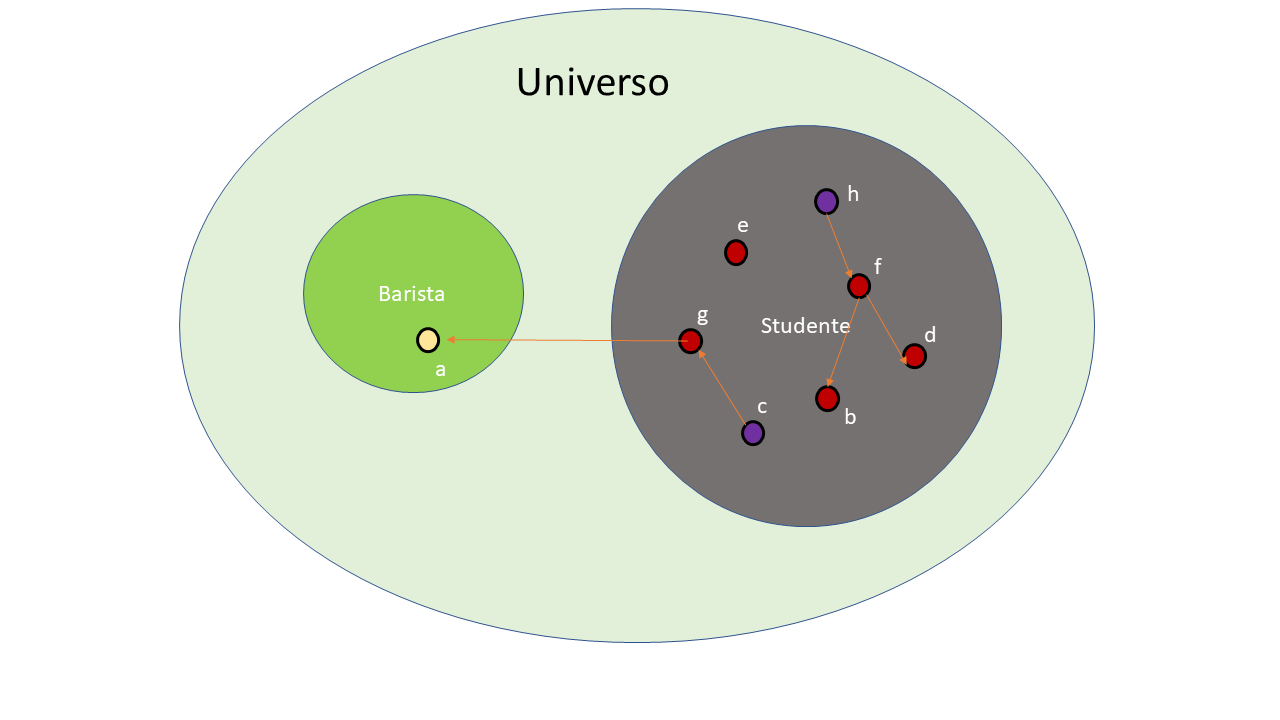
\includegraphics[width=\textwidth]{FdiValutazione.png}
	\label{fig:valutaz}
	\centering
\end{figure}
\clearpage
Intuitivamente un individuo \textit{m} è \textbf{tipico} se non esiste alcun elemento più \textit{normale},
viceversa, un  \textit{n} è \textbf{atipico} quando esiste almeno un individuo più \textit{normale}.
Indichiamo formalmente che l'espressione:
\begin{itemize}
	\item[] \makebox[4cm]{$ x < y $} (l'individuo $ x $ è più \textit{normale} di $ y $)
\end{itemize}
Consideriamo dunque l'esempio \ref{fig:valutaz} della pagina precedente:\\
gli studenti tipici sono $ b,c,d,e,f,g,h $, in particolare, $ e $ è tipico perché non è in alcuna
relazione del tipo $ x < y $, per quanto riguarda la catena$  h, f, d, b $ si evince che $ d $ e $ b $ siano più
\textit{normali} di $ f $ che a sua volta è più \textit{normale} di $ h $;\\ 
come conseguenza $ d $ e $ b $ risultano essere tipici poiché questa catena non prosegue bensì termina con loro due. 
Invece non risulta corretto concludere che $ g $ sia uno studente tipico, infatti, nonostante sia 
più normale di $ c $, è in relazione con $ a $, tuttavia $ a $ appartiene 
ad un insieme diverso (Barista) e questo non influisce sulla sua "tipicità".
La relazione di preferenza ha limite di essere parziale, 
infatti non è sempre possibile stabilire quale elemento sia più tipico degli altri.

In realtà l’estensione di questa sezione viene chiamata $ \mathcal{ALC + \mathbf{T_{R}}} $ dove il pedice
R indica il concetto di logica razionale sulle cui proprietà si basa la semantica di
T. Tali caratteristiche, come la \textit{specificità}, costituiscono le fondamenta del ragionamento non monotono, 
permettendo modellare la situazione in questo modo:

\begin{figure}[h]
	\caption{Un esempio di modello}
	\label{fig:esempioM}
	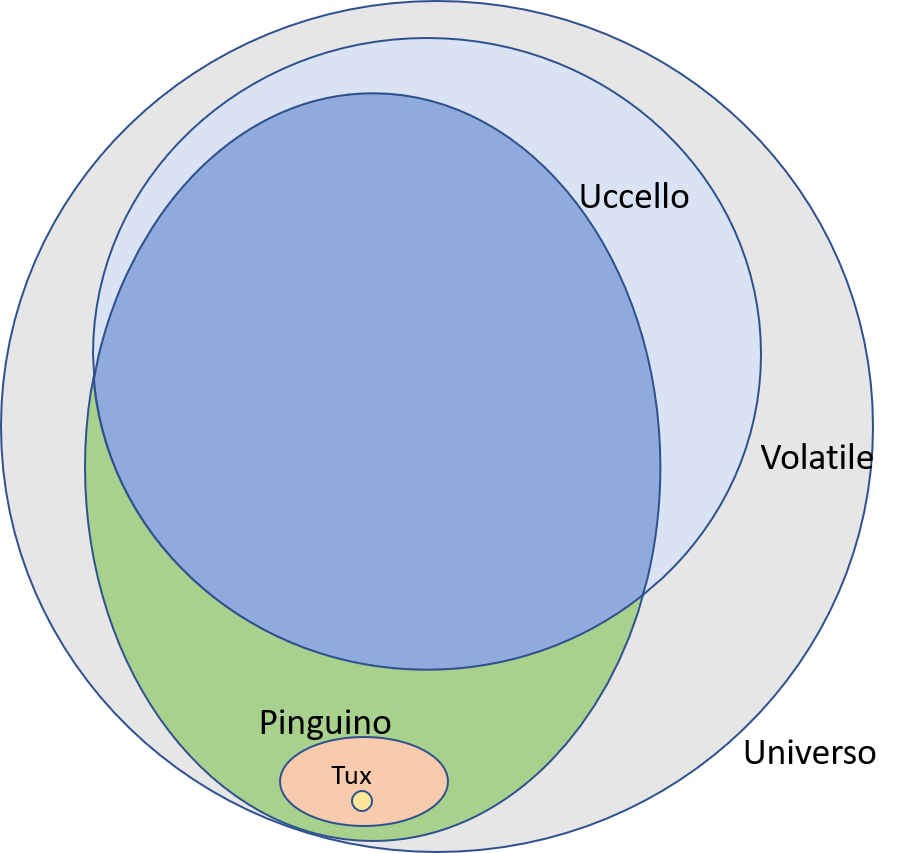
\includegraphics[height=13cm,width=\textwidth]{immagini/ModelloALC_T.png}
	\centering
\end{figure}
Nella Figura \ref{fig:esempioM} è possibile rappresentare Tux (un \textit{Pinguino}) come è un uccello che non vola;
graficamente quest'informazione è racchiusa nella zona verde dell'insieme Uccello,
ovvero, quella sezione popolata da tutti gli uccelli atipici, mentre la porzione in blu rappresenta gli elementi tipici.

\section{La logica non monotona $ \mathcal{ALC} + \mathbf{T}_{\mathbf{R}}^{\mathit{RaCl}} $}
Nonostante l'aggiunta dell'operatore $ \mathbf{T} $ la logica appena vista rimane monotona, 
nel senso che se il fatto $ F $ segue da una certa base
di conoscenza \textbf{KB} , allora lo stesso fatto $ F $ segue da una qualsiasi $ KB' \subseteq KB $. 
Di conseguenza, a meno che una base di conoscenza contenga delle assunzioni esplicite circa la tipicalità degli individui, non esiste alcun modo per inferire proprietà rivedibili su di loro. \\
Un'altra limite riguarda l'intrattabilità della \textit{irrilevanza}.
\begin{itemize}
	\item[] $ LottatoreDiSumo \sqsubseteq Atleta $
	\item[] $ \mathbf{T}(Atleta) \sqsubseteq \neg Grasso $
	\item[] $ \mathbf{T}(LottatoreDiSumo) \sqsubseteq Grasso $
\end{itemize}
per via della monotonia di $ \mathcal{ALC + \mathbf{T_{R}}} $ non si può derivare che:
\[ \mathbf{T}(LottatoreDiSumo \sqcap Orientale) \sqsubseteq Grasso \] 
malgrado l'etnia sia totalmente irrilevante rispetto all'essere grassi o magri.

Con l'obbiettivo di creare inferenze non monotone utili gli autori in \cite{FromPLtoDL} hanno rinforzato la semantica precedente restringendo le assegnazioni ad una classe minimale di modelli. 
L’idea è quella di restringere l’assegnazione a modelli minimi che \textit{minimizzino l'atipicalità dei concetti} e
dove le inclusioni implicate sono quelle che appartengono alla chiusura razionale della base di conoscenza, 
estensione naturale di \cite{Conditional_KB}.

Considerare solo i modelli che massimizzano le istanze tipiche di un concetto quando sono 
consistenti con la base di conoscenza.
Senza entrare troppo nei dettagli la semantica $\mathcal{ALC} + \mathbf{T}_{\mathbf{R}}^{\mathit{RaCl}}$
non monotona si basa su modelli razionali minimi che riducono al minimo il \textit{rank} degli elementi del dominio.

Intuitivamente, dati due modelli $ \mathcal{M_1,M_2} $ di una \textbf{KB} se è noto che 
in $ M_1 $ un elemento $ x $ ha rank 2 (a causa di istanze $ z < y < x $) ed
in $ M_2 $ $ x $ ha rank 1 (a causa di $ y < x $), noi preferiamo il secondo,
perché l’elemento x risulta più tipico che in $ M_1 $.
I modelli vengono quindi selezionati per il ragionamento scartando quelli grado più elevato poiché in essi gli elementi sono meno "tipici" e quindi verrebbero dedotte meno informazioni (vedi anche Figura a pagina \pageref{fig:valutaz}).

\clearpage

\subsection{Traduzione dell'operatore T} \label{subSec: Traduzione T}
In alcuni contesti non è sempre possibile modificare l'intera struttura basata su logiche consolidate.
È sensato chiedersi quale sia il significato di questo operatore e se esistano formulazioni equivalenti.
Consideriamo la \textit{TBox}:
\[ \mathbf{T}(Pesce) \sqsubseteq Oviparo \]
Come sappiamo esprime il fatto che, tipicamente, gli uccelli sono ovipari (depositano le uova). \\
Ecco la traduzione equipollente, vista in \cite{PEAR} e \cite{COCOS}, senza far uso dell'operatore $ \mathbf{T} $ è la seguente: 
\begin{enumerate}\label{enu:elencoCond}
	\item $ Pesce \sqcap Pesce1 \sqsubseteq Oviparo $
	\item $ Pesce1 \sqsubseteq \forall R(\neg Pesce \sqcap Pesce1) $
	\item $ \neg Pesce1 \sqsubseteq \exists R(Pesce \sqcap Pesce1) $
\end{enumerate} 
Questa traduzione implementa la relazione d'ordine $ < $ precedentemente introdotta.\\
L'insieme $ Pesce1 $ rappresenta i pesci tipici mentre $ Pesce $ contiene tutti i possibili pesci, 
compresi quelli atipici, e costituisce infatti un soprainsieme di Pesce1. \\ 
La suddivisione in questi due insiemi a \ref{fig:tradPesce} è fondamentale per poter tenere traccia delle eccezioni, ottenendo così la possibilità di ragionare sia sull'individuo generico sia sul tipico individuo.\\
\begin{figure}[h]
	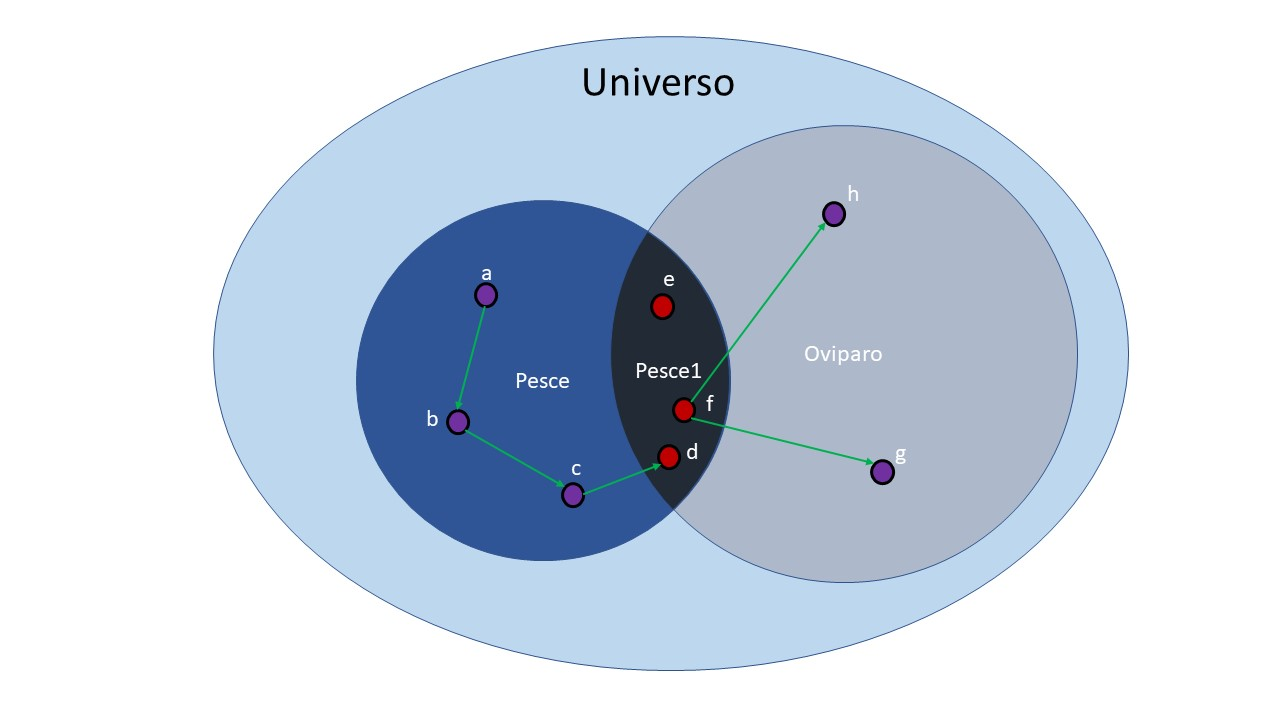
\includegraphics[width=\textwidth]{Traduzione_T_.jpg}
	\centering
	\caption{Esempio traduzione $ \mathbf{T}(Pesce) \sqsubseteq Oviparo $}
	\label{fig:tradPesce}
\end{figure}
Pertanto per inferire che $ nemo $ sia un tipico $ Pesce $ controllerà che la seguente espressione sia vera:
\[ \mathbf{T}(Pesce)(nemo) \iff Pesce(nemo) \land Pesce1(nemo) \]

In caso di risposta affermativa sarà verificato che: 
\[ Pesce(nemo) \sqcap Pesce1(nemo) \sqsubseteq Oviparo(nemo) \]

Ecco quindi verificata la condizione $ 1 $ di \ref{enu:elencoCond}
Viceversa la definizione $ 2 \text{ e } 3 $ esprimono formalmente cosa significhi essere un individuo a/tipico.
\begin{multicols}{2}
	$ Pesce1 \sqsubseteq \forall R.(\neg Pesce \sqcap Pesce1) $ \\
	$ \neg Pesce1 \sqsubseteq \exists R.(Pesce \sqcap Pesce1) $
\end{multicols}
Nell'esempio \ref{enu:elencoCond}, i membri $ d,e \text{ ed } f $ sono pesci tipici. È evidente che l'intersezione
$ \neg Pesce \sqcap Pesce1 $ sia vuota. Dunque deduciamo che, dato l'insieme $ A $, se un elemento $ m \in A$ 
è \textbf{tipico} o non è in alcuna relazione del tipo $ x < y $ ()e quindi non esiste un 
individuo più normale di lui) o è più ordinario di un generico $ x $ $(m < x)$ con $ x \in A $ 
oppure si trovi nella relazione $ x < m $ dove però $ x \notin A $.

Per quanto concerne i pesci \textbf{atipici}, come le istanze $ a,b \text{ e } c $, per verificarne la tipicità 
viene svolto un procedimento molto simile. Prendiamo in esempio $ b $: viene verificato inizialmente lo stato
dell'elemento (se si trovi o meno in una o più relazioni) e analizzato. In questo caso scopriamo che è più 
caratteristico di $ a $ ma meno di $ c $ che, a sua volta, è più generico di $ d $, che scopriamo essere tipico.
Per transitività troviamo la relazione $ d < b $ che conferma a b la sua atipicità.
In conclusione, un membro è atipico quando esiste \textbf{almeno un} individuo più normale di lui

\section{La logica $ \mathcal{ALC} + \mathbf{T}_{\mathbf{R}}^{\mathtt{P}} $}
Dopo aver illustrato la logica di base $ \mathcal{ALC} $ ed introdotto l’estensione non monotona
$ \mathcal{ALC} + \mathbf{T} $ con i relativi concetti di \textbf{chiusura e logica razionale}, in questa sezione
verrà descritta l’estensione "accennata" nel capitolo introduttivo \ref{itemize: 3 comp} che permette di tenere in considerazione la probabilità di individui particolari \cite{ProbOfEx}.

\subsection{Modifiche alla semantica }
L'inclusione di tipicalità si evolve e va ad assumere la forma:
\[ \mathbf{T}(C) \sqsubseteq_{p} D \]
con il significato intuitivo aggiuntivo: la probabilità di avere un $ C $ eccezionale (cioè \textbf{atipico})
che non sia anche un $ D $ vale $ 1-p $.

La base di conoscenza (\textbf{KB}) $ (TBox,ABox) $ ha la seguente struttura
\begin{multicols}{2}
	$ TBox $ in cui $ p \in \mathbb{} e p \in (0,1) $
	\begin{itemize}
		\item $ C \sqsubseteq_{p} P $
		\item $ \mathbf{T}(C) \sqsubseteq_{p} P $
	\end{itemize} 
	$ ABox $ in cui $ a,b \in \mathcal{0} $
	\begin{itemize}
		\item $ C(a) $
		\item $ R(a,b) $
	\end{itemize}
\end{multicols}

È facilmente intuibile che più la probabilità p è alta più l’inclusione è "libera da eccezioni" o, 
equivalentemente, è meno probabile avere un C speciale che non è anche un D.\\
A tal proposito è importante sottolineare che la probabilità $ p $  con $ p = 1 $ non è consentita 
in quanto l’inclusione $ \mathbf{T}(C) \sqsubseteq_{1} D  $
corrisponde all'inclusione stretta $ \mathbf{T}(C) \sqsubseteq D $ che esprime invece il fatto che
l’elemento $ C $ è sicuramente anche un $ D $.\\
Data una seconda inclusione $ \mathbf{T}(C') \sqsubseteq_{p'} D' $, con $ p' < p $, si assume che questa
inclusione sia meno "restrittiva" rispetto alla prima in quanto la possibilità di avere un
eccezionale $ C' $ è più alta rispetto alla probabilità di avere un eccezionale $ C $, tenendo rispettivamente
conto delle proprietà $ D' \text{ e } D $.

Considerando, per esempio, la seguente \textit{TBox}
\begin{itemize}
	\item $ \mathbf{T}(Liceale) \sqsubseteq_{0.80} Studioso $
	\item $ \mathbf{T}(Liceale) \sqsubseteq_{0.60} PraticaDelloSport $
\end{itemize}
si evince che il tipico scolare è studioso e che, normalmente, pratica dello sport;
entrambe sono proprietà del prototipo dello studente, tuttavia ci sono più
eccezioni di studenti che non fanno sport rispetto a quelli che non studiano.

Una cosa importante da tenere in considerazione è la possibilità di avere \textit{Knowledge Base}
contenenti inclusioni con $ p \leq 0.5 $, che se
erroneamente interpretate, potrebbero venir considerate contro-intuitive.

Ad esempio,l’inclusione $ \mathbf{T}(Liceale) \sqsubseteq_{0.22} Fumatore  $  potrebbe venir erroneamente 
interpretata come "normalmente, gli studenti non sono fumatori"; anche se la corrispondente probabilità è bassa, 
la spiegazione corretta è che fare uso di sigarette è in ogni caso una 
proprietà del prototipo dello studente liceale.\\
A differenza dell'espressione $ \mathbf{T}(Liceale) \sqsubseteq_{0.80} Studioso $, si ha che la
probabilità di trovare studenti eccezionali non fumatori è più alta rispetto a quella
di trovare studenti eccezionali che siano studiosi.\\
%ma entrambe sono tipiche proprietà di uno studente.
Ponendo il caso in cui si volesse formalizzare che il tipico studente non è una persona giovane, bisogna 
semplicemente formulare l’inclusione $ \mathbf{T}(Liceale) \sqsubseteq_{0.78} \neg Fumatore  $ nella base di conoscenza.

\subsection{Estensione dell'\textit{Abox}}
Data una base di conoscenza \textbf{KB }, viene definito l’insieme finito $ \mathfrak{Tip} $ dei concetti che
occorrono all'interno dell'operatore di tipicalità, formalmente
\[ \mathfrak{Tip} = \{ C | \mathbf{T}(C) \sqsubseteq_{p} D \in KB \}. \]
Dato un individuo $ a $ esplicitamente dichiarato nell'\textit{ABox}, si definisce l’insieme delle
assunzioni di tipicalità $ \mathbf{T}(C)(a) $ che possono essere dedotte in maniera minimale dalla \textbf{KB}
nella logica non monotona $ \mathcal{ALC} + \mathbf{T}_{\mathbf{R}}^{\mathit{RaCl}} $, con $C \in \mathfrak{Tip}$.

Quindi si considera un insieme ordinato $ \mathfrak{Tip}_{\mathcal{A}}$ (dove $ \mathcal{A} $ sta per \textit{ABox})
di coppie $ (a, C) $ di tutte le possibili assunzioni $ \mathbf{T}(C)(a) $, 
per tutti i concetti $ C \in \mathfrak{Tip} $ e per tutti gli individui $ a $ nell'\textit{ABox}.

In aggiunta si definisce il multi-insieme ordinato $ \mathcal{P_{A}}$ tupla della forma $[p_1,p_2,...,p_n] $
dove $ p_i $ è la probabilità dell'assunzione $ \mathbf{T}(C)(a) $ tale che $ (a,C) \in 
\mathfrak{Tip}_{\mathcal{A}} $ alla posizione $ i $; inoltre rappresenta il prodotto di tutte le probabilità 
$ p_ij $ delle inclusioni $ \mathbf{T}(C) \sqsubseteq_{p_ij} D $ nella \textit{TBox}.

%Da rivedere wide tilde
Seguendo le idee di \cite{ReasoningOnScen}, si considerano diverse estensioni $ \mathcal{\widetilde{A}}_i $
dell'\textit{ABox} che vengono equipaggiate con una probabilità $ p_i $. Partendo dagli insiemi  
$ \mathcal{P_{A}} = [p_1,p_2,...,p_n] $ e $ \mathfrak{Tip}_{\mathcal{A}}$, il primo passo è quello 
di definire l'insieme $ \mathbb{S} $ di tutte le stringhe di possibili assunzioni, utilizzando lo 0 come $ p_i $ per rappresentare che la corrispondente asserzione di tipicalità non viene più assunta.

Successivamente, si definisce l’estensione $ \mathcal{\widetilde{A}}_i $ di $ \mathcal{{A}} $ 
corrispondente ad una stringa $ [s_1,s_2,...,s_n] \in \mathbb{S} $ cosi ottenuta. 
In questo modo, la probabilità più alta viene assegnata all'estensione dell'\textit{ABox} corrispondente a 
$ \mathcal{P_{A}} $, dove tutte le assunzioni di tipicalità vengono considerate.
mentre diminuisce nelle altre estensioni, alcune assunzioni di tipicalità vengono scartate, 
così 0 viene usato al posto della corrispondente $ p_i $.

La probabilità di una estensione quindi $ \mathcal{\widetilde{A}}_i $ corrispondente a 
$ \mathcal{P_{A}}_i  = [p_{i1},p_{i2}, . . . ,p_{in}] $ è definita come il prodotto delle probabilità 
$ p_{ij} $ quando $ p_{ij} \neq 0 $ ( cioè la possibilità della corrispondente assunzione di 
tipicalità nel momento in cui questa viene selezionata per l’estensione) e $ 1 - p_j $ quando $ p_{ij} = 0 $ (cioè la corrispondente assunzione di tipicalità viene scartata, per segnalare che 
l’estensione contiene un’eccezione all'inclusione).

Si può osservare che, in $ \mathcal{ALC} + \mathbf{T}_{\mathbf{R}}^{\mathit{RaCl}} $, 
l’insieme delle assunzioni di tipicalità che
possono essere inferite da una \textbf{KB} corrispondono all'estensione $ \mathcal{A} $ equivalenti alla
stringa $ \mathcal{P_{A}} $ (nel caso in nessun elemento sia impostato a 0);
vengono considerate tutte le assunzioni di tipicalità,
degli individui presenti nell’\textit{ABox}, consistenti con la base di conoscenza.\\
Al contrario, in $ \mathcal{ALC} + \mathbf{T}_{\mathbf{R}} $, nessuna assunzione di tipicalità può esser dedotta
da una \textbf{KB}, e questo equivale ad estendere $ \mathcal{A} $ con delle asserzioni corrispondenti alla
stringa $ [0, 0, . . . , 0] $, ovvero l'insieme vuoto.

Otteniamo dunque una distribuzione di probabilità sulle estensioni di $ \mathcal{A})$ (se presenti).
Prendiamo come esempio una $ \textbf{KB} (\mathcal{T} , \mathcal{A}) $ in cui le uniche 
inclusioni di tipicalità in $ \mathcal{T} $ siano le seguenti:
\begin{enumerate}
	\item $ \mathbf{T}(C) \sqsubseteq_{0.60} D $
	\item $ \mathbf{T}(E) \sqsubseteq_{0.85} F $
\end{enumerate}
e $ a $ e $ b $ siano gli unici individui presenti in $ \mathcal{A} $; supponiamo inoltre che $ \mathbf{T}(C)(a) $, 
$ \mathbf{T}(C)(b) $ e $ \mathbf{T}(E)(b) $ siano dedotte dalla \textbf{KB} con la logica 
$ \mathcal{ALC} + \mathbf{T}_{\mathbf{R}}^{\mathtt{P}} $.

Il risultato è quindi:
\begin{multicols}{2}
	$ \mathfrak{Tip}_{\mathcal{A}} = \{(a,C),(b,C),(b,E)\} $ \\
	$ \mathcal{P_{A}} = [0.6, 0.6, 0,85] $
\end{multicols}
Tutte le possibili stringhe, tutte le corrispondenti estensioni di $ \mathcal{A} $ e tutte le probabilità 
sono illustrate nella seguente tabella \ref{fig:estesioni}
\clearpage
\begin{figure}[t]
	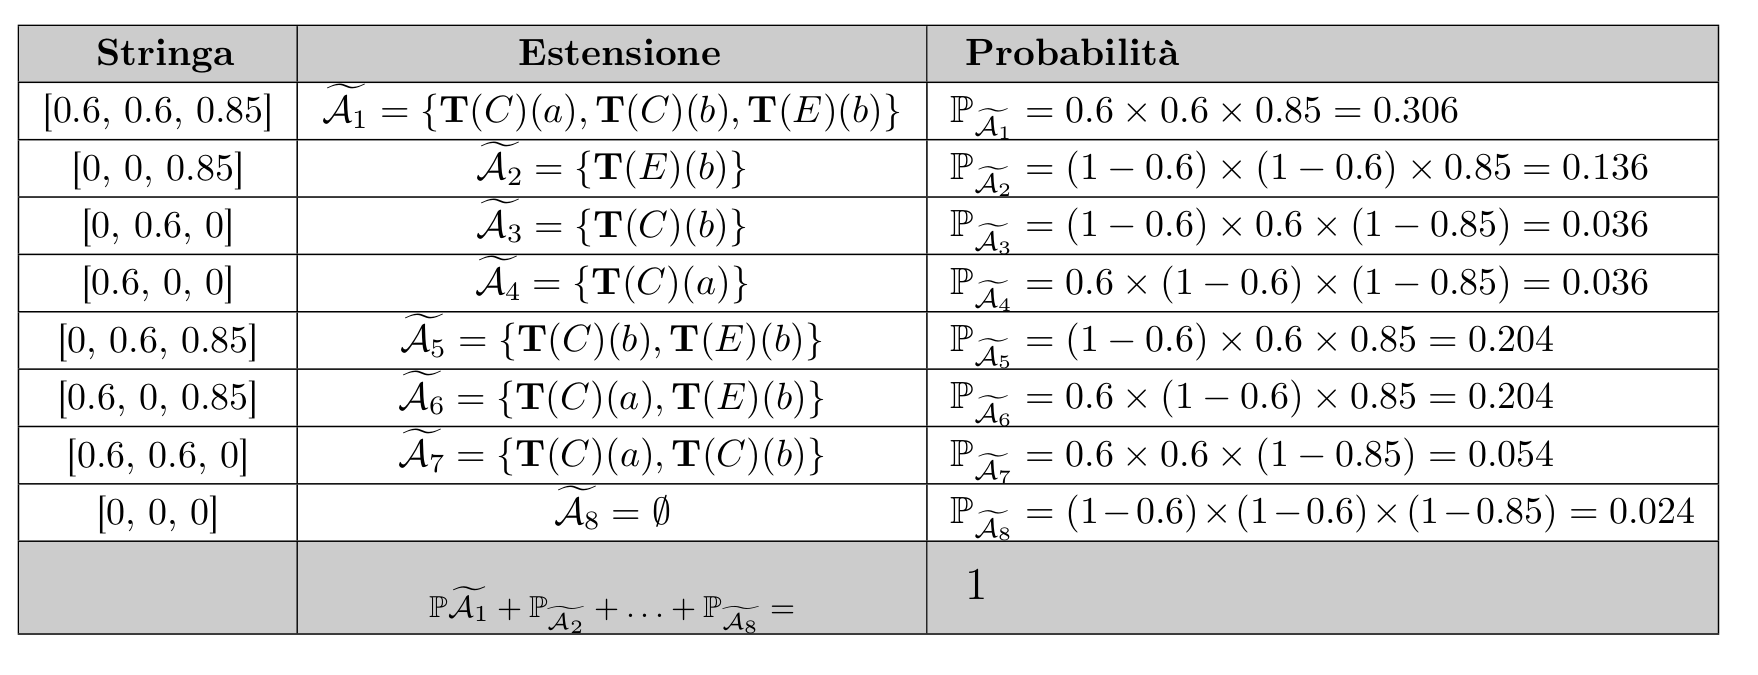
\includegraphics[width=\linewidth]{Estensione_Plausibile.png}
	\caption{Estensioni plausibili}
	\label{fig:estesioni}
	\centering
\end{figure}

\subsection{Dalla logica verso la "diagnosi"}
Descriviamo formalmente cosa si intenda per diagnosi in questo contesto particolare, aiutandoci con un esempio.
Data la seguente \textbf{KB} con \\ $ \textit{ABox} = \{MemoryLoss(Pietro)\} $ e \textit{TBox}:
\begin{itemize}
	\item $ Paranoia \sqsubseteq Depressed $
	\item $ \mathbf{T}(AlzheimerPatient) \sqsubseteq_{0.85} MemoryLoss $
	\item $ \mathbf{T}(AlzheimerPatient) \sqsubseteq_{0.65} Paranoia $
	\item $ \mathbf{T}(DiabetesPatient) \sqsubseteq_{0.90} Thirst $
	\item $ \mathbf{T}(DiabetesPatient) \sqsubseteq_{0.55} Depressed $
	\item $ \mathbf{T}(Depressed) \sqsubseteq_{0.80} Insomnia $
	\item $ \mathbf{T}(Depressed) \sqsubseteq_{0.70} Headache $
\end{itemize}

consideriamo un set $ \mathcal{V} $, espresso nella forma $ C(a) $, che rappresenta i sintomi e i segni nella forma:
\[ \mathcal{V} = \{ Paranoia(Pietro), Headache(Pietro) \} \]
sappiamo che  $ \mathcal{V} $ non è implicato dalla base di conoscenza, ma che $ \textbf{KB} \sqcup \mathcal{V} $ è \textit{consistente}.
Utilizzando la  logica $ \mathcal{ALC} + \mathbf{T}_{\mathbf{R}}^{\mathtt{P}} $ siamo interessati a trovare 
una diagnosi per i sintomi di $ Pietro $, cioè un insieme di \textit{asserzioni} $ D $ tali che $ \textbf{KB} \sqcup D \models \mathcal{V} $.\\
Seguendo l'esempio:
\begin{itemize}
	\item $ D_1 = \{AlzheimerPatient(Pietro)\} $ \textbf{segue logicamente}
	\item $ D_2 = \{Depressed(Pietro)\} $ \textbf{non segue logicamente}
	\item $ D_3 = \{AlzheimerPatient(Pietro), Depressed(Pietro)\} $ \textbf{segue logicamente}
\end{itemize}
che corrispondono a
\begin{itemize}
	\item \makebox[5,5cm]{$ \mathbf{T}(AlzheimerPatient)(Pietro) $\hfill} è implicato da $ \textbf{KB} \sqcup D_1 \land \textbf{KB} \sqcup D_3 $
	\item \makebox[5,5cm]{$ \mathbf{T}(Depressed)(Pietro) $ \hfill} è implicato solo in $ \textbf{KB} \sqcup D_3 $
	\item \makebox[5,5cm]{$ \mathbf{T}(DiabetesPatient)(Pietro) $ \hfill} non è implicato da nessuna \textbf{KB}
\end{itemize}
Possiamo ragionare sugli scenari, consideriamo, ad esempio, $ D_3 $ con 
\[ \mathfrak{Tip}_{\mathcal{A}} = {(Pietro,AlzheimerPatient), (Pietro,Depressed)} \] 
e con $ \mathcal{P_{A}} = [0.525,0.556] $ dove $ 0.525 = 0.85 \times 0.65 $ è la probabilità di equipaggiare
la proprietà tipica del concetto $ AlzheimerPatient $, discorso analogo per $ Depressed $.
Utilizzando quanto visto precedentemente si considerano le seguenti estensioni
\begin{itemize}
	\item \makebox[13.97cm]{$ \mathcal{\widetilde{A}}^3_1 = \{\mathbf{T}(AlzheimerPatient)(Pietro)\} $\hfill} 
		con $ \mathcal{P_{\widetilde{A}^\mathit{3_1}}} =  0.525 \times 0.463 = 0.243 $
	\item \makebox[13.97cm]{$ \mathcal{\widetilde{A}}^3_3 = \{\mathbf{T}(AlzheimerPatient)(Pietro), \mathbf{T}(Depressed)(Pietro)\} $ \hfill}
		con $ \mathcal{P_{\widetilde{A}^\mathit{3_3}}} = 0.556 \times 0.557 = 0.309  $
\end{itemize}
deduciamo, dunque, che:
\[ \textbf{KB} \sqcup D_i \models (\mathcal{ALC} + \mathbf{T}_{\mathbf{R}}^{\mathtt{P}}) ^{(0,1)} Paranoia(Pietro), Headache(Pietro) \]
con $ i = 1,3 $, vale a dire che tutte le asserzioni di cui sopra rappresentano una diagnosi per i sintomi $ \mathcal{V} $

E con questo concludiamo la trattazione dei fondamenti di logica.\\ 
Questa capitolo altro non è che un sunto, a tratti informale, della storia di questa branca matematica  
e non sostituisce certamente gli articoli e studi fatti nel corso degli anni, da figure molto più autorevoli,
della mia ma costituisce il corpo fondante di tutta la tesi.





	
	\chapter{Strumenti utilizzati}
	In questo capitolo descriveremo le componenti che utilizzeremo nella nostra
architettura e, per ognuna di queste, introdurremo brevemente le caratteristiche chiave.
\section{OWL2}

L'OWL 2 Web Ontology Language, informalmente OWL 2, è un linguaggio ontologico per il Semantic Web con un significato formale e definito \cite{OWl2Primer}.\\
Le ontologie in OWL 2 vengono definite tramite la specifica di classi, proprietà, individui e valori dei dati e sono memorizzate come documenti del Semantic Web.
Queste possono essere pubblicate sul web e riferite da altre ontologie, per costruire basi di conoscenza più complesse. 
Inoltre sono spesso utilizzate assieme insieme a documenti scritti nel formato RDF, ed stesse vengono scambiate principalmente come documenti RDF.

\subsection{Semantica}
La semantica è definita \textit{formalmente}, cioè permette di scrivere \textit{Knowledge Base} sulle quali è possibile applicare inferenze in modo automatico.
OWl2 possiede due semantiche:
\begin{itemize}
	\item[] \textbf{Semantica diretta}, basata sulle Logiche Descrittive (vedi pag.\pageref{chap: DL})
		\begin{itemize}
			\item è applicabile a un frammento del linguaggio detto OWL2 DL;
			\item è sempre decidibile;
			\item ha una sintassi più ristretta. 
		\end{itemize}
	\item[] \textbf{Semantica Indiretta}, basata sui grafi RDF
		\begin{itemize}
			\item estende la semantica formale di RDF
			\item ha la massima espressività 
			\item la decibilità non garantita
		\end{itemize}
\end{itemize}
la sēmantikós è basata su \textbf{iff} (se e solo se) quindi:
\[ C \text{ è sottoclasse di D } \iff  \text{istanze di } C \subseteq \text{istanze di } D \]

\subsection{Caratteristiche}
Il linguaggio prevede tre componenti principali:
\begin{enumerate}
	\item \textbf{Entità}: elementi atomici usati per riferirsi ad oggetti, categorie e relazioni 
	del mondo reale; costituiscono gli assiomi\\ 
	$Lara,donna,Pietro,Sofia,essere_fidanzati$ 
	\item \textbf{Assiomi}: affermazioni (\textit{statement}) di base espressi da un'ontologia OWL
	$Lara$ è una $donna$ | $ Pietro $ e $ Sofia $ sono $ fidanzati $
	\item \textbf{Espressioni}: combinazioni di entità che costituiscono descrizioni complesse, definite
	tramite l'utilizzo di costruttori. \\
	$ Medico $ e $ Donna $ combinate definiscono $ Donna Medico $ 
\end{enumerate}
 
Ogni file \textit{.owl} inizia con un preambolo: \label{code:preambolo}
\begin{minted}{XML} 
	Prefix(:=<http://example.com/owl/families/>)
	Prefix(otherOnt:=<http://example.org/otherOntologies/families/>)
	Prefix(xsd:=<http://www.w3.org/2001/XMLSchema#>)
	Prefix(owl:=<http://www.w3.org/2002/07/owl#>)
	Ontology(<http://example.com/owl/families>
	Import( <http://example.org/otherOntologies/families.owl> )
	....
\end{minted} 
\mint{XML}|Prefix(..)| permette di fare, sinteticamente, riferimento a elementi definiti in altre ontologie o in altri file; il prefisso più l'etichetta sono composti nell'identificatore dell'elemento di interesse, ad esempio
\mintinline{XML}{owl:Thing} diventa \mintinline{XML}{http://www.w3.org/2002/07/owl#Thing}.
\mint{XML}|Ontology(..)| Specifica l'\textbf{URI} (Uniform Resource Identifier) del file contenente l'ontologia
definita
\subsection{Sintassi e Modellazione di Base} \label{subSec: SintassiOWL}
È possibile scrivere ontologie OWL utilizzando sintassi differenti:
\begin{itemize}
	\item Functional-Style \mintinline{XML}{ClassAssertion(:Persona:Damiano)}
	\item Manchester \mintinline{XML}{Individual: Damiano}
	\item Turtle \mintinline{XML}{:Damiano rdf:type :Persona}
	\item RDF/XML \mintinline{XML}{<Persona rdf:about="Damiano">}
	\item OWL \begin{minted}{XML}
	<ClassAssertion>
	<Class IRI="Person"/>
	<NamedIndividual IRI="Damiano"/>
	</ClassAssertion>
	\end{minted}
\end{itemize}
Ed esiste una chiara equivalenza tra le varie terminologie utilizzate, vediamola:
\begin{multicols}{3}
	\textit{Ing. della conoscenza}
	\begin{itemize}
		\item Oggetti 
		\item Categorie 
		\item Relazioni
	\end{itemize}
	\textit{Description Logic}
	\begin{itemize}
		\item Costanti
		\item Predicati Unari 
		\item Predicati Binari
	\end{itemize}
    \textit{Termini OWL}
	\begin{itemize}
		\item Individui
		\item Classi 
		\item Proprietà
	\end{itemize}
\end{multicols}
Dopo queste considerazioni generali, entriamo ora nei dettagli della modellazione con OWL2.
Nei paragrafi successivi introdurremo le funzionalità essenziali per produrre una base di conoscenza. Queste saranno condite con esempi,
semplici dimostrazioni delle varie funzionalità di OWL.
Per semplicità useremo il \textit{Functional-Style}.

Ecco come si esprimono gli Assiomi: 
\begin{itemize}
	\item dichiarazioni di individuo: \mintinline{XML}{Declaration(Name Individual(:Dario))}
	\item dichiarazioni di classe: \mintinline{XML}{Declaration(Class(:Persona))}
	\item dichiarazioni di proprietà: \mintinline{XML}{Declaration(ObjectProperty(:Uomo))}
\end{itemize}
E alcune delle relazioni chiave:

\makebox[8cm]{\mintinline{XML}{ClassAssertion(:Persona :Dario))} \hfill} lega un'istanza ad una classe; \\
\makebox[8cm]{\mintinline{XML}{SubClassOf(:Persona :Uomo))} \hfill} relazione di sottoclasse ($ \sqsubseteq $); \\
\makebox[8cm]{\mintinline{XML}{EquivalentClasses(:Persona :Umano)}\hfill} equivalenza di due classi;\\
\makebox[8cm]{\mintinline{XML}{DisjointClasses(:Donna :Uomo)}\hfill} classi disgiunte.

Permette di legare due individui tramite una proprietà.
\mint{XML}{ObjectPropertyAssertion(:haMoglie :Donna :Uomo)}
\subsection{Classi complesse e implementazione di $ \cap,\cup,\exists $ e $ \forall $}
Tramite opportuni costrutti è possibile specificare classi complicate e relazionarle, 
anche grazie all'operatore di intersezione $\cap$ e disgiunzione $ \cup $.
\begin{minted}{XML}
	EquivalentClasses(:Padre
		ObjectIntersectionOf(:Uomo :Genitore))
	EquivalentClasses(:Genitore
		ObjectIntersectionOf(:Madre :Padre))
\end{minted}
Nonna è sottoclasse dell'intersezione fra \textit{Donna e Genitore}.
\begin{minted}{XML}
	SubClassOf(:Nonna 
		ObjectIntersectionOf(:Donna :Genitore))
\end{minted}
L'individuo \textit{Marco} è una \textit{Persona} (e) non \textit{Genitore}.
\begin{minted}{XML}
	ClassAssertion(
		ObjectIntersectionOf(:Persona 
			ObjectComplementOf(:Genitore))
	:Marco)
\end{minted}
Vediamo, infine, come si possa utilizzare i quantificatori $ \exists $ e $ \forall $ con qualche esempio.
La classe \textit{Genitore} è l'insieme di quegli individui che possiedono almeno un'istanza 
di \textit{Persona} che è loro Figlio; una persona è \textit{Felice} quanto tutti 
i suoi figli sono felici. Le persone che non hanno figli, vengono inclusi come felici.
\begin{multicols}{2}
	Quantificatore esistenziale $ \exists $
	\begin{minted}{XML}
	EquivalentClasses(
	  :Genitore
	  ObjectSomeValuesFrom
	  (:haFiglio :Persona))
	\end{minted}
	
	Quantificatore universale $ \forall $
	\begin{minted}{XML}
	EquivalentClasses(
	  :PersonaFelice
	   ObjectAllValuesFrom
	    (:haFiglio :PersonaFelice))
	\end{minted}
\end{multicols}

Questo conclude la nostra breve visione sintetica del linguaggio.

\subsection{OWl2 \emph{Versus} DB e considerazioni finali}
I file \textit{.owl} conservano informazioni ma nonostante ciò OWL2 \textbf{non} è un framework
per basi di dati; Nonostante parte della terminologia evochi assonanze con i \textbf{D}ata\textbf{B}ase, 
la semantica di base ha delle differenze sostanziali.

In primis l'assunzione di mondo: un fatto non contenuto in un \textbf{DB} è considerato falso (mondo chiuso) mentre nel mondo
logico viene considerato mancante (mondo aperto). In secondo luogo, classi e proprietà possono avere definizioni multiple e OWL non richiede che le uniche proprietà di un individuo siano quelle della classe a cui appartiene.
Infine ricordiamo ciò che abbiamo visto a \ref{code:preambolo} : le informazioni riguardanti un singolo individuo 
possono essere distribuite su più documenti diversi, contrariamente ad un classico \textbf{DB}.

In conclusione vogliamo ricordare che OWL \textbf{non} è un linguaggio di programmazione, bensì
un linguaggio \textit{dichiarativo}, in grado di rappresentare della conoscenza. Diversi sono gli strumenti
a disposizione per trattare le ontologie: ragionatori automatici, API, validatori, editor e ambienti di sviluppo.
Nella sezione successiva tratteremo alcuni di questi tool che fanno parte di DbN.  

\section{Owlready2} \label{sec: OwlR2}
Lavorare direttamente con OWL è impegnativo e tedioso, ma, in nostro soccorso, arrivano le API (Application Programming Interface).
Tra le più recenti e interessanti spicca Owlready2 \cite{OwlReady}, pratica libreria \textit{ontology-oriented}, scritta in Python3. Owlready versione 2 permette un accesso trasparente alle ontologie, contrariamente alle API basate su Java.
Può caricare ontologie OWL2 come oggetti Python, modificarli, salvarli e, appoggiandosi ad  \textit{HermiT} e \textit{Pellet} (reasoner scritti in Java), eseguire veri e propri ragionamenti.
Vediamo alcune caratteristiche chiave

\subsection{Tabella di conversione}
Se dovessimo "convertire" le formule tra Description Logics, Owlready2 e/o Protegè,
potrebbe essere di interesse la sottostante tabella.

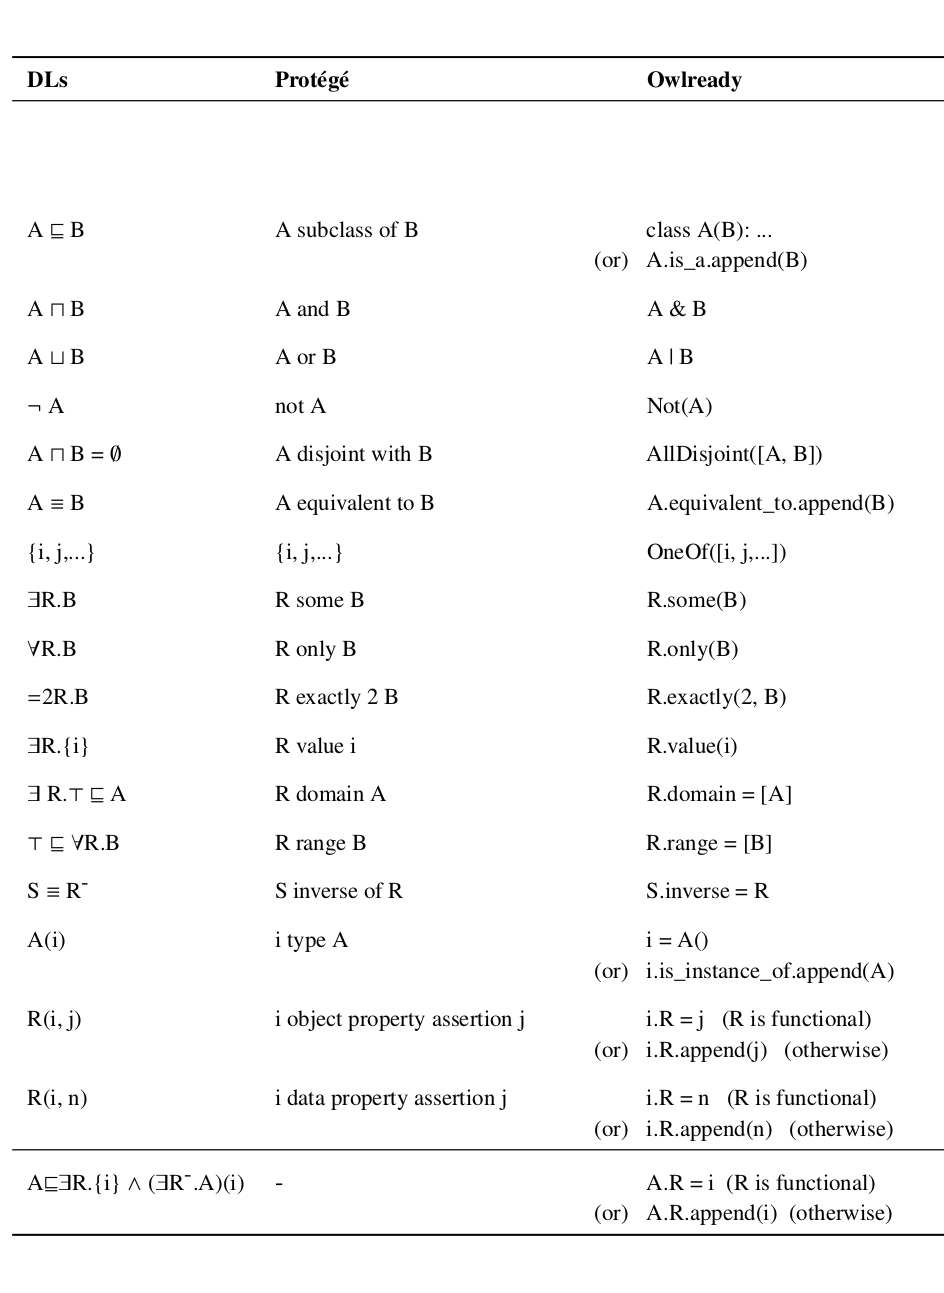
\includegraphics[width=\linewidth]{immagini/ConversionTable.png}

Molti di questi simboli ci sono familiari e, di conseguenza, 
il salto rappresentazionale è molto basso.
Utilizzare la semantica di questo pacchetto non risulta troppo impegnativo, poiché coerente
con le Logiche Descrittive.

\subsection{Che cosa posso fare con OWLReady2?}
\inputminted{Python}{codice/IntroOwlReady2.py}

\subsection{Architettura}
Owlready2 mantiene un quadstore (\textbf{DB} di quadruple) RDF in un database ottimizzato \textit{SQLite3}, sia in memoria che, opzionalmente, su disco.\\
Fornisce, inoltre, un accesso di alto livello alle classi e agli oggetti presenti 
nell'ontologia. Classi e Individui vengono caricati dinamicamente dal \textbf{DB} secondo
necessità, salvati in memoria e poi eliminati quando non più necessari.

\subsection{Paragone con precedenti approcci}

\begin{figure}[h]
	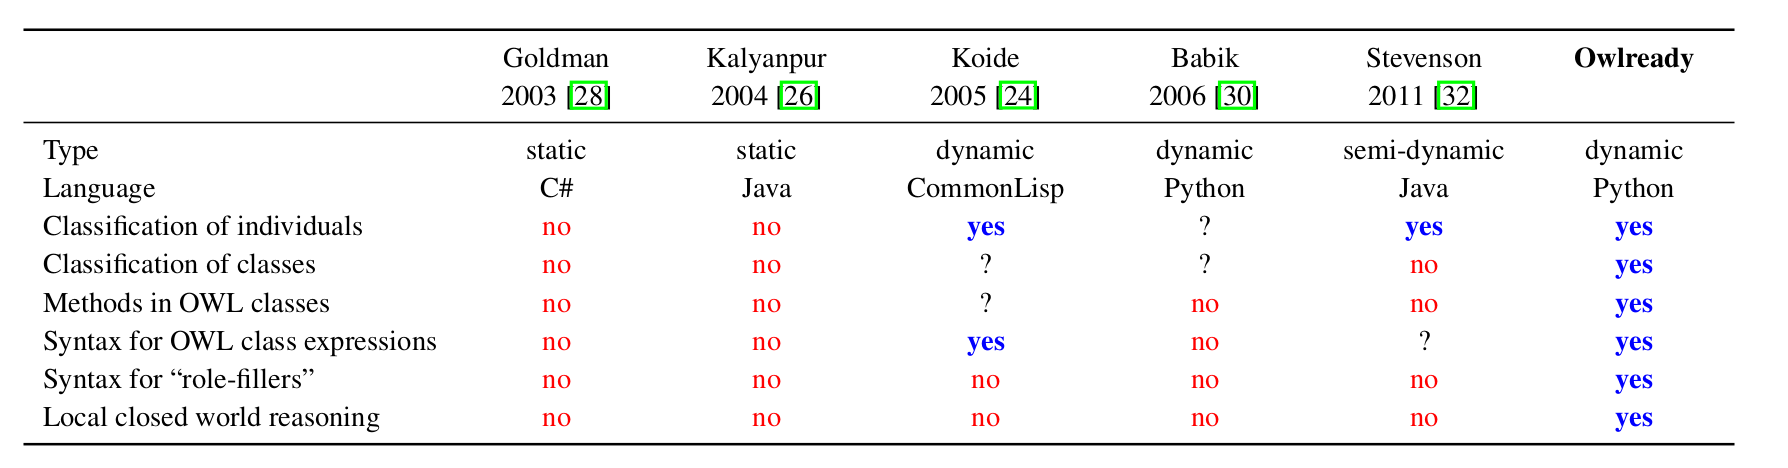
\includegraphics[width=\linewidth]{Tabella_Comp_Owlr2.png}
	\caption{Paragone di Owlready con altri approci di programmazione.}
	\centering
	\label{fig:tabComparativa}
\end{figure}

La tabella \ref{fig:tabComparativa} confronta diverse tecnologie precedenti con Owlready2.
Owlready si distingue come uno degli approcci più avanzati. In particolare,
è in grado di classificare automaticamente (non solo gli individui ma anche le classi),
compiere "reasoning" sul mondo locale chiuso e non e proporre una sintassi ad alto livello per
definire i vincoli "role-fillers". Queste ed altre caratteristiche risultano cruciali quando
si lavora con ontologie mediche, ma posso essere utili anche in altri domini.

Questo sono le componenti chiave di un sistema capace di adattarsi a
differenti casi d’uso in maniera decisamente flessibile

\section{Plotly} \label{sec: Plotly}
Plotly.py è una delle migliori librerie \textit{Open Source} di plotting: supporta oltre 40 tipi di grafici unici, 
interattivi e ricchi di funzionalità, andando a coprire una vasta gamma di casi d'uso: statistico, finanziario, geografico, 
scientifico e tridimensionale. Non mancano i classici grafici a linee, a barre, a bolle e a punti. \cite{Plotly}

\subsection{Perché usare Plotly.py?}
Costruita sopra la più celebre libreria Javascript (Plotly.js, composta da d3.js e stack.gl), 
Ploty.py permette di creare bellissime realizzazioni interattive basate sul web, che possono
essere salvate come file HTML o utilizzate come parte di web-app scritte in Python.
Tutti i grafici di Plotly.py sono completamente costumomizzabili. 
Tutto, dai colori e dalle etichette alle linee della griglia e alle legende, può essere personalizzato 
utilizzando una serie di attributi dedicati.
I diagrammi, inoltre, sono dotati di funzionalità interessanti come lo zoom, il panning, il ridimensionamento automatico, ecc. \\
Grazie all'integrazione profonda con Orca, utility per l'esportazione di immagini, Plotly.py
fornisce un notevole supporto anche per i contesti al di fuori del web, inclusi gli IDE (PyCharm, Spyder)
e la pubblicazione di documenti cartacei, come questo testo.

L'obiettivo era quello di rendere gradevoli ed esplicativi i risultati "diagnostici" prodotti dal tool DbN.

\subsection{Che cosa posso fare con Plotly.py?}
\inputminted{Python}{codice/IntroPlotly.py}







	
	\chapter{Caso d'uso: Tool per il supporto diagnostico}
	\chaptermark{Caso d'uso}
	In questo capitolo verrà descritto il programma oggetto della tesi DbN (Diagnosis by Numbers) che altro 
non è che un'estensione di \textbf{PEAR} (Probability of Exceptions and typicAlity Reasoner) \cite{PEAR}.
Inizialmente si fornirà un breve riassunto del lavoro di Soriano; successivamente cosa sia stato preso o meno.\\
Poi obiettivi posti e aggiunte ed infine il progetto completo con annesso esempio.
Come linguaggio per lo sviluppo è stato scelto \emph{Python} (in particolare la sua
versione \textit{Python3.7}) per diversi motivi, eccone alcuni:
\begin{itemize}
	\item continuità con il lavoro precedente;
	\item la presenza di nuove API (vedi \ref{sec: OwlR2} pag. \pageref{sec: OwlR2});
	\item tipicamente richiede meno codice rispetto ad altri;
	\item è uno dei linguaggi più popolari per l'elaborazione scientifica;
\end{itemize}

\section{PEAR - Sintesi}
\paragraph{Struttura}Questo tool, basato sulla logica $ \mathcal{ALC} + \mathbf{T}_{\mathbf{R}}^{\mathtt{P}} $, è strumento 
che permette di ragionare e dedurre informazioni, di definire 
precisamente chi siano gli individui tipici, atipici e quali siano
le caratteristiche peculiari di una data categoria.
Il funzionamento dell'intero strumento è riassumibile in questi passi:
\begin{enumerate}
	\item dopo aver letto le informazioni costituenti la KB, presenti in un file a parte, 
	viene creata l’ontologia;
	\item vengono combinate le probabilità delle assunzioni di tipicalità e generati tutti 
	gli scenari (possibili realtà dei fatti);
	\item di ogni scenario viene calcolata la probabilità complessiva;
	\item viene verificata o meno la consequenzialità logica del fatto $ F $ dato in input per ogni scenario;
	\item infine vengono mostrati i risultati dell'interrogazione.
\end{enumerate}
Questo è possibile anche grazie alla seguente architettura:
\begin{figure}[ht]
	\centering
	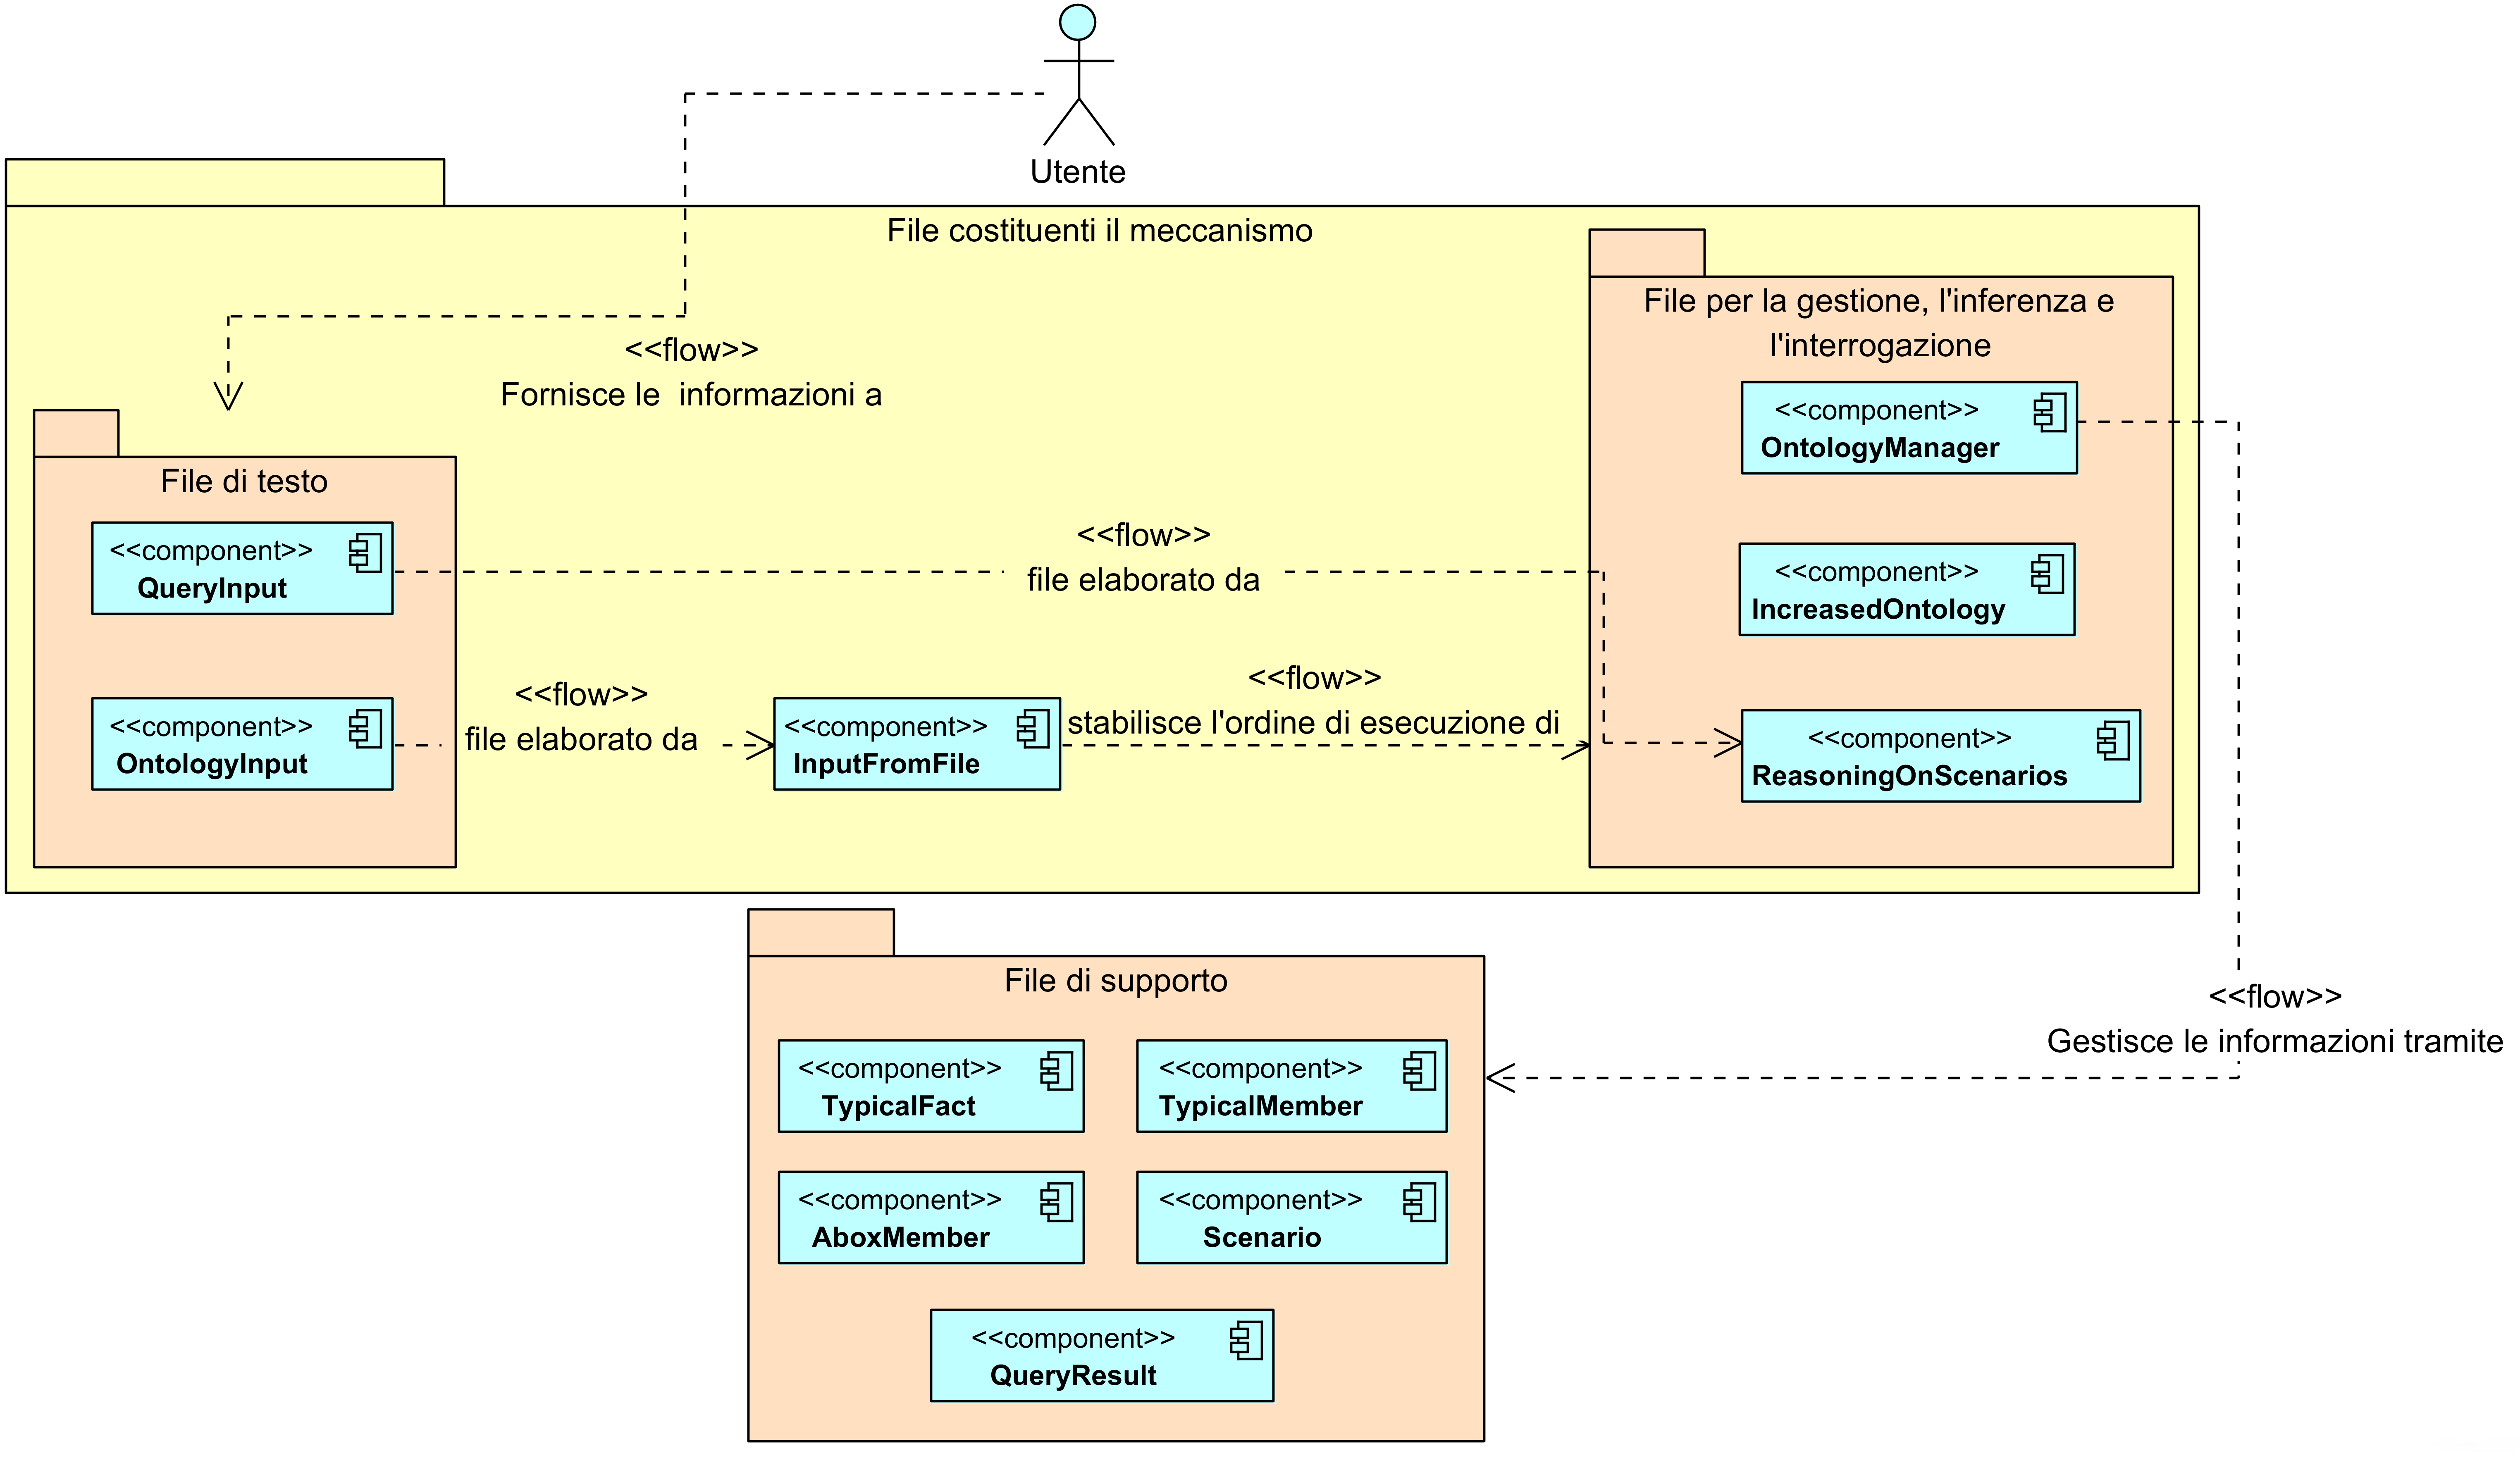
\includegraphics[width=\linewidth]{immagini/architetturaPEAR.png}
	\caption{Archittetura di Pear}
\end{figure}
dove i singoli file richiamano, spesso, i concetti teorici associati, precedentemente illustrati.
\paragraph{Limiti}
Le conclusioni così prodotte sono certamente interessanti, ma la procedura di ragionamento in se è vincolata, di volta
in volta, dalla query iniziale. \\Intuitivamente, ci si chiede se un determinato evento $ F $ sia 
conseguenza logica nella possibili diramazioni (scenari) $ B_1,B_2,....,B_n $ della base di conoscenza $ B $.
Questo procedimento non è applicabile in un contesto realistico, poiché chiederebbe all'utente di comprendere
la logica anche solo per capire come effettuare un'interrogazione significativa.
Inoltre sono presenti dei difetti tecnici, come, ad esempio, la necessità, durante la verifica di
conseguenza logica, di effettuare una copia dell'istanza del manager dell'ontologia per ogni scenario.

Alla luce di quanto detto in precedenza ecco la necessità di ottimizzazione ed espansione di PEAR in 
una naturale evoluzione: \textsl{Diagnosis by Numbers}

\section{Visione complessiva}
L'idea di questa tesi, introdotta nel capitolo 1 e ribadita più volte, finalmente inizia a prender forma.
Data un'ontologia, più o meno vasta, arricchita da espressioni di tipicalità e dai sintomi/prodromi
riguardanti un paziente, l'obiettivo è quello di generare tutte le possibili diagnosi (o spiegazioni),
controllarne la veridicità (logicamente parlando) e presentarle in forma grafica, evidenziandone la 
probabilità e il costo stimato.

Ovviamente il focus principale rimane la correttezza di esecuzione, non tanto la complessità dell'ontologia
medica o dei costi diagnostici reali. Questo non toglie che in futuro possa avere delle applicazioni concrete.

\paragraph{Struttura del progetto}
Il progetto è composto da 12 File; questi, a volte, verranno indicati con un intuitiva abbreviazione, 
così da rendere la lettura più scorrevole:
\begin{itemize}
	\item \emph{Main.py} file principale, contenente l'ordine d'esecuzione delle operazioni.
	\item Due file di testo, di input:
	\begin{itemize}
		\item \emph{OntologyInput.txt} contiene classi, relazioni tra classi, fatti tipici
			ed individui; 
		\item \emph{PatientSetOfSymptoms.txt} composto da coppie individuo-classe.
	\end{itemize}
	\item Quattro file chiave:
	\begin{itemize}
		\item \emph{OntologyManager.py} gestisce tutto ciò che riguarda l'ontologia;
		\item \emph{InputFromFile.py} si occupa della traduzione del file OntoInput tramite OntoManager;
		\item \emph{IncreasedOntology.py} calcola le probabilità di ogni membro tipico e genera tutti gli scenari;
		\item \emph{ReasoningOnScenarios.py} calcola le probabilità per ogni scenario ed effettua il ragionamento per ogni scenario arricchito con gli scenari.
	\end{itemize}
	\item Cinque file di supporto:
	\begin{itemize}
		\item \emph{AboxMember.py} corrispettivo dell'\textit{ABox};
		\item \emph{TypicalFact.py} assieme alla classe TypicalMember\\ corrispettivo dell'\textit{TBox};
		\item \emph{TypicalMember.py} assieme alla classe TypicalFact\\ corrispettivo dell'\textit{TBox};
		\item \emph{Scenario.py} rappresenta il singolo scenario;
		\item \emph{QueryResult.py} memorizza i risultati e genera il grafico associato.
	\end{itemize}
\end{itemize}
Le successive sezioni del capitolo andranno ad illustrare le funzionalità chiave dello strumento organizzate per file.
\section{Immissione dei dati}
\subsection{I documenti in ingresso}
Partiamo dall'illustrare come vengano memorizzate le informazioni relative all'ontologia dallo strumento 
e quale sia il corrispettivo del file in termini di logiche descrittive. 
\inputminted[lastline=11]{text}{codice/ExOntoInput.txt}
Il file \emph{OntologyInput.txt} è composto da 4 parti:\\
\begin{enumerate}
	\item \mintinline{text}{Classes} altro non è che un elenco di tutte le classi che si andranno ad utilizzare;
	\item \mintinline{text}{Set_as_sub_class} è una lista composta da coppie sottoclasse e classe, vedi il sottoparagrafo \ref{subSec: SintassiOWL};
	\item \mintinline{text}{Add_members_to_class} contiene gli individui e le relative classi di appartenenza; 
	\item \mintinline{text}{Set_typical_facts:} contiene l'elenco delle inclusioni di tipicalità.
\end{enumerate}

La stessa ontologia espressa in termini di \textbf{KB}$ (\mathcal{T}, \mathcal{A}) $:
\begin{itemize}
	\item $\mathcal{TB}ox$ 
		\begin{itemize}
			\item $ Bipolar \sqsubset Depressed $
			\item $ \mathbf T(ProstateCancerPatient) \sqsubseteq_{0.80} Nocturia $
			\item $ \mathbf T(Depressed) \sqsubseteq_{0.85} \neg MoodReactivity $
		\end{itemize}
	\item $\mathcal{AB}ox$ 
		\begin{itemize}
			\item $ Depressed(Greg) $
			\item $ ProstateCancerPatient(Luca) $
		\end{itemize}
\end{itemize}

In fondo al documento troviamo un nuovo elemento, i costi diagnostici; ogni malattia tipica avrà
un costo associato e, alla fine dell'elaborazione, verranno elaborati e combinati per assegnare al singolo
scenario un costo indicativo, al fine di dare un ulteriore criterio di preferenza al medico.
\inputminted[firstline=13]{text}{codice/ExOntoInput.txt}
Sotto \mintinline{text}{Set_cost_of} vi sono le coppie malattia-costo stimato (in €)

Infine il file \emph{PatientSetOfSymptoms.txt} in confronto è più basilare
\begin{minted}{text}
	Luca;Not(Bipolar) | Greg;Nocturia
\end{minted} 
Questi fatti verranno manipolati e poi aggiunti all'$ Abox$ in ogni scenario, solo se consistenti con l'ontologia di base.

\subsection{La classe dedicata alla traduzione} \label{subSec: InputFile}
Il file \emph{InputFromFile.py} contiene due metodi:
\mintinline{Python}{build_ontology} e \mintinline{Python}{read_symptoms}.
Ogni metodo si occupano del rispettivo file, rispettivamente \emph{OntologyInput.txt} e \emph{PatientSetOfSymptoms.txt}.
Infatti, dopo aver letto il contenuto del file di testo,
le stringhe vengono elaborate e successivamente data in input ai metodi della classe \mintinline{Python}{OntologyManager} quali 
\mintinline{Python}{create_class, add_sub_class_, add_member_to_class} ecc.
Come ulteriore ottimizzazione, l'esecuzione di \mintinline{Python}{read_symptoms} viene effettuata una sola volta, poiché
si è preferito salvare i dati letti in \mintinline{Python}{dict()} (coppie chiave-valore) dedicato tramite il metodo
\mintinline{Python}{store_for_reasoning}, che vedremo più in dettaglio nella prossima sezione.

Rispetto alla versione precedente il codice è stato ottimizzato e reso più leggibile anche grazie all'introduzione
di due funzioni ausiliare \mintinline{Python}{strip_not} e \mintinline{Python}{strip_typical}.
Come si intuisce dal nome lo scopo di queste 1-line-function è di rimuovere le stringhe \mintinline{Python}{"Not"}
e \mintinline{Python}{"Typical"} che son superflue e vanno diversamente gestite.

\section{L' amministrazione dell'ontologia}
Nel file \emph{OntologyManager.py}, contenente l'omonima classe, sono presenti numerosi metodi per
la creazione e la gestione dei mondi e delle ontologie. Focalizziamo la nostra attenzione sul costruttore:
\begin{minted}{Python}
def __init__(self, iri="http://www.example.org/onto.owl"):
	self.typical_facts_list = list()
	self.a_box_members_list = list()
	self.scenarios_list = list()
	self.typical_members_list = list()
	self.cost_dict = dict()
	self.symptoms_dict = dict()
	self.my_world = World()
	self.big_world = World()
	self.onto = self.my_world.get_ontology(iri)
\end{minted}
notiamo, oltre alla presenza dell'iri \ref{subSec: SintassiOWL}, l'utilizzo di una variabile, dal nome esplicativo, 
per ogni lista necessaria. La novità più importante riguarda l'utilizzo dei mondi. \textit{Owlready2 }
\ref{sec: OwlR2} può supportare numerosi mondi isolati, e questo ci aiuta, poiché siamo interessati a caricare
diverse versioni della stessa ontologia. Ecco quindi spiegate le due differenti variabili.
\mintinline{Python}{my_world} è utilizzata per contenere l'ontologia di base, mentre
\mintinline{Python}{big_world} ha lo scopo di racchiudere l'ontoBase arricchita con lo scenario selezionato.
Se non si capisce ora quale sia l'utilità di questa scelta, successivamente verrà illustrata in maniera più approfondita.

Passiamo ora ad analizzare i metodi di istanza incaricati della gestione dell'ontologia; la maggior parte sono semplici wrapper delle risorse fornite dalla libreria e non richiedono ulteriori spiegazioni. Tuttavia, 
tra questi spiccano i metodi per la gestione dei \textit{fatti tipici} e dei \textit{membri tipici}, 
operatori non conosciuti dalla nostra \textbf{API} di Python.
La soluzione migliore, già adotta in PEAR, consiste nell'eliminare l'operatore $ \mathbf T $ tramite una
particolare traduzione, vista a \ref{subSec: Traduzione T} e implementata nel metodo 
\mintinline{Python}{add_typical_fact}.
Ricordiamo, brevemente, che un paziente è atipico quando esiste \textbf{almeno un} individuo più normale di lui.
Per, invece, esprimere il concetto di membro $ m $ è un tipico $ C $ bisogna dire che $ m $ appartiene sia
alla classe $ C $ (tutti gli elementi) sia alla classe $ C1 $ (elementi tipici).
Questa idea trova la sua realizzazione nel metodo \mintinline{Python}{set_as_typical_member}.

Per ridurre i tempi di lettura e manipolazione da file si è voluto introdurre una mappa dedicata ai sintomi
con due funzioni manipolative associate, vediamole: 
\begin{minted}{Python}
def store_for_reasoning(self, member_name: str, class_id: object):
	self.symptoms_dict.update({class_id: member_name})

def add_symptoms_to_kb(self):
	for class_sy, pname, in self.symptoms_dict.items():
		class_c = self.create_class(class_sy.name)
		not_class_c = self.create_class("Not(" + class_sy.name + ")")
		class_c.equivalent_to = [Not(not_class_c)]
		self.add_member_to_class(pname, not_class_c, symp=True)
		print("Sintomo aggiunto: " + pname + ": " + class_c.name)
\end{minted}
la prima ha il compito di aggiungere valori al "dizionario" le coppie:\\ \mintinline{Python}{nome-paziente: classe-sintomo}.\\
La seconda, invece, per ogni coppia presente nella struttura, crea le classi appropriate e poi 
aggiunge un membro all'\textit{ABox} all'ontologia corrente tramite la funzione \mintinline{Python}{add_member_to_class}.

È altrettanto importante focalizzarci sulla gestione dei mondi, effettuata dai metodi:
\begin{minted}{Python}
	def save_base_world(self):
	 self.onto.save("ontoBase.owl", format="ntriples")
	
	def create_new_world(self):
	 self.onto.destroy()
	 self.big_world = World()
	 self.onto = self.big_world.get_ontology(
	 "file://" + PATH_TO_ONTO + "//ontoBase.owl").load() 
\end{minted}
il primo possiede l'incarico di esportare l'ontologia, creata nell'omonimo mondo nel punto 
\ref{subSec: InputFile}
Il secondo assume la funzione di distruggere l'ontologia contenuta nella variabile \textit{onto}, 
di creare un nuovo mondo e di caricare l'ontologia salvata precedentemente sul file.
Vedremo meglio più avanti quale sia stata la strategia dietro lo sviluppo di questi metodi.\\
Analogamente a questo concetto citiamo la seguente funzione:
\begin{minted}{Python}
def consistency(self, condition: bool = False):
	try:
	with self.onto:
		if condition:
			sync_reasoner(self.my_world)
			classi_incosistenti = list(
 				self.my_world.inconsistent_classes())
			if not len(classi_incosistenti) == 0:
 				return classi_incosistenti
		else:
			sync_reasoner(self.big_world)
   		return "The ontology is consistent"
	except OwlReadyInconsistentOntologyError:
 		return "The ontology is inconsistent"
\end{minted}
I ragionatore \emph{Hermit} è in grado di controllare la consistenza di un ontologia e dedurre nuovi fatti,
riclassificando individui e classi in base alle loro relazioni. In caso di inconsistenza viene lanciata
l'eccezione appropriata. È possibile avere classi inconsistenti senza rendere l'intera ontologia
inconsistente ,a patto che queste non abbiano individui. In nostro aiuto il reasoner inferisce tali classi
come equivalenti to \textbf{Nothing} (elemento primitivo di OWL) ed è quindi possibile interrompere 
l'esecuzione del tool prima che l'intera ontologia sia inconsistente!
Vediamo un esempio. Se avessi una \textbf{KB}:
\begin{multicols}{2}
	\textit{TBox}
	\begin{itemize}
		\item $ \neg A \sqsubseteq B $
		\item $ B \sqsubseteq A $
		\item $ \mathbf{T}(C) \sqsubseteq_{0.80} D $
	\end{itemize}
	\columnbreak
	\textit{ABox}
	\begin{itemize}
		\item $ D(Giovanni) $
	\end{itemize}
\end{multicols}
La classe $ \neg A $, nonostante non abbia elementi, è inconsistente poiché in contraddizione con
l'assioma $ B \sqsubseteq A $. Questo chiude la trattazione del manager.

\section{La creazione dei membri tipici e degli scenari}
Il file \emph{IncreasedOntology.py} è un modulo che fornisce i metodi necessari per la
generazione di tutti i membri tipici e gli scenari possibili e per il calcolo delle relative probabilità.
I metodi incaricati del valutazione delle "percentuali" sono:
\begin{minted}{Python}
def compute_probability_for_typical_members(onto_manager):
	facts_list = onto_manager.typical_facts_list
	abox_members_list = onto_manager.a_box_members_list
	facts_list.sort(key=lambda x: x.t_class_identifier.name)
	abox_members_list.sort(key=lambda x: x.class_identifier.name)
	......
    __set_probability( prob_to_assign_to_typical_member, onto_manager,
    	facts_list[i].t_class_identifier,
    	facts_list[i].class_identifier)
	....
	
def __set_probability(prob_to_assign, onto_mng, t_class_id, class_id):
	for aboxMember in onto_mng.a_box_members_list:
		if aboxMember.isSymptom is True and
		 aboxMember.class_identifier.name == class_id.name:
			onto_mng.typical_members_list.
			append(TypicalMember(
				t_class_id,
				aboxMember.member_name,
				prob_to_assign
			))
\end{minted}
Il primo processo è il più complicato e si avvale del secondo come supporto.
In sintesi per computare la probabilità da associare ad ogni membro tipico si 
vanno a moltiplicare tra loro le probabilità di ogni inclusione di tipicalità avente la
medesima classe argomento dell’operatore $ \mathbf{T} $
(ovvero \mintinline{Python}{t_class_identifier}) e, a quel punto, il metodo
di supporto,viene invocato per creare il membro tipico.

Ricordiamo che $ m $ è tipico se è nella forma $ p:\mathbf{T}(C)(m) $.
Tale funzione, quindi, scansionando tutti i membri dell'\textit{ABox}, cerca quello che è un sintomo
e ha come classe di appartenenza $ C $. Una volta trovato, passa alla creazione Membro tipico, con la 
probabilità calcolata precedentemente.

La seconda parte della classe ha la responsabilità degli scenari, realtà possibili dei fatti.
Il numero totale cambia al variare dei \mintinline{Python}{TypicalMember} e del numero di Sintomi,
in particolare, con $ n $ membri tipici è $ 2^{n} $. Considerando, ad esempio, $ mt1 $ e $ mt2 $
l'insieme risultante sarà la combinazione:
\[ \{\{\emptyset\},\{mt1\},\{mt2\},\{mt1,mt2\}\} \]
dove $ \emptyset $ rappresenta lo scenario vuoto, in cui non si fa alcuna assunzione, $ \{mt1\} $
in cui si assume solo $ mt1 $, $ \{mt2\} $ in cui si assume solo $ mt2 $ e infine l'ultimo 
dove si assumono entrambi.

Per quanto riguarda la probabilità da associare ad ogni scenario, essa è data dal 
prodotto di $ k $ fattori, con $ k $ pari al numero di membri tipici generati (nell’esempio
precedente avendo due \mintinline{Python}{TypicalMember}, la probabilità di ognuno dei 
quattro scenari è data dal prodotto di $ k = 2 $ fattori) dove ogni fattore è una probabilità 
che coincide con la $ p $ appartenente al membro tipico  se assunto, 
altrimenti vale $ 1 - p $ se questo, nello scenario, non viene assunto.\\
Riprendendo l’esempio precedente, supponendo che $ mt1 $ abbia come probabilità il valore $ p1 $ 
e che $ mt2 $ abbia il valore $ p2 $, la probabilità dello scenario vuoto vale $ ( 1 - p1) \ ( 1 - p2)$,
quella dello scenario in cui si assume solo $ mt1 $ vale $ p1 \times ( 1 - p2) $, 
quella in cui si assume solo $ mt2 $ vale $ ( 1 - p1) \times p2 $ ed infine l’ultimo scenario $ p1 \times p2 $.

I metodi che si occupano di questa traduzione sono 4, 1 principale e 3 di supporto "privati":
\begin{minted}{Python}
def set_probability_for_each_scenario(ontology_manager):
def __generate_scenario(ontology_manager):
def __difference(scenario, typical_members_list):
def __get_typical_member(key, ontology_manager):
\end{minted}
Per prima cosa il metodo \mintinline{Python}{set_probability_for_each_scenario} 
genera tutti gli scenari tramite il metodo \mintinline{Python}{__generate_scenario} (determinando
l’insieme delle parti), successivamente gli scenari vengono così processati:
viene moltiplicata la probabilità dei membri tipici assunti e non assunti 
(grazie a \mintinline{Python}{__difference}) in modo da calcolare la probabilità per ogni scenario.
Questo verrà memorizzato nell'oggetto dedicato \mintinline{Python}{Scenario}
 ovviamente gestito dall'\mintinline{Python}{OntologyManager}.

In particolare il metodo \mintinline{Python}{__difference} effettua una 
differenza insiemistica tra i due insiemi: membri tipici: assunti e generati. 
\mintinline{Python}{__get_typical_member}, invece, calcola la probabilità del membro tipico non assunto
nello scenario corrente grazie alla presenza delle chiavi identificative \mintinline{Python}{key}:
cerca all'interno dell'\mintinline{Python}{ontology_manager} l’oggetto \mintinline{Python}{TypicalMember} corrispondente a quella chiave.

Abbiamo deciso di ignorare lo scenario $ \emptyset $ poiché è il più banale, già scartato in altri contesti.
Infatti è corretto logicamente generare tale scenario ma, verificato o meno se sia conseguenza logica della KB,
non ha molto senso dare una diagnosi del tipo: con una probabilità X non ha niente.

\section{L'inferenza}
Il file \emph{ReasoningOnScenarios.py} si occupa di verificare se i sintomi in input
seguano logicamente dalla base di conoscenza, arricchita con l'aggiunta di un determinato scenario.
Questo per ogni oggetto \mintinline{Python}{Scenario} presente.
Per verificare l'\textit{implicazione logica}, in simbolo $  A \models B $, bisogna verificare che
in tutti i modelli in cui $ A $ è $ True $, anche $ B $ è vera. Nel nostro caso dobbiamo provare
che $ KB \cup S \models V $ dove $ S $ è un determinato scenario e $ V $ è un set di formule che
rappresenta i sintomi del paziente. Possiamo dimostrare ciò grazie 
alla dimostrazione per \textbf{refutazione}, che permette di
rispondere $ True $ se si dimostra l'equivalenza $ (KB \cup S \wedge\neg V) \equiv False $.
DbN utilizzerà proprio questa strategia, vediamo come.
\begin{minted}{Python}
def __translate_scenario(scenario, ontology_manager):
	for tm in scenario.list_of_typical_members:
		ontology_manager.set_as_typical_member(
			tm.member_name, tm.t_class_identifier, 
			ontology_manager.
			onto[tm.t_class_identifier.name + "1"])
def is_logical_consequence(ontology_manager, 
	lower_probability_bound=0, higher_probability_bound=1):
\end{minted}
Il metodo, di supporto, \mintinline{Python}{translate_scenarios} ha il compito di tradurre 
ogni membro tipico presente all’interno dello scenario.
Il metodo \mintinline{Python}{is_logical_consequence} gestisce l'intera fase di verifica, 
opzionalmente esaminando solo gli scenari in un determinato intervallo di probabilità, tramite
gli argomenti facoltativi lower and higher \mintinline{Python}{_bound}.
I risultati verranno salvati all'interno di \mintinline{Python}{query_result = QueryResult()}.
Una volta selezionati gli scenari, questi vengono esaminati uno per volta nel seguente modo:
\begin{enumerate}
	\item viene creato un nuovo \mintinline{Python}{mondo}, un'universo isolato, in cui si carica
	 	l'ontologia di base creata in precedenza;
	\item a questa vengono aggiunti i sintomi \textbf{negati} e lo scenario corrente, tramite i metodi
	 \mintinline{Python}{add_symptoms_to_kb()} e \mintinline{Python}{__translate_scenario()};
	\item quindi si verifica la consistenza dell'ontologia:
	\begin{itemize}
		\item se è consistente, cioè $ \equiv True $, allora $ KB \cup S \not\models V $ 
			e quindi lo scenario viene ignorato e il ciclo riparte \textbf{loop}.
	\end{itemize}
	\item In caso contrario, si salva l'oggetto \mintinline{Python}{Scenario} 
		all'interno di \mintinline{Python}{query_result};
	\item e si accumula la probabilità dello scenario, appena verificato, \\
		nella var \mintinline{Python}{total_probability}, riparte il \textbf{loop}; 		
\end{enumerate}
Alla fine del ciclo si salva la probabilità totale così all'interno della variabile\\ \mintinline{Python}{query_result}. L' esecuzione quindi termina.

\section{Analisi del risultato}
Alla luce di quanto detto prima, vediamo ora la struttura del file \emph{QueryResult.py} e, 
in particolare, delle sue operazioni.
\begin{minted}{Python}
def show_query_result(self):
	.....
def create_and_show_plot(self, patient_symptoms: str, disease_cost: dict):
	# Crea una figura con un secondo asse y
	self.fig = make_subplots(specs=[[{"secondary_y": True}]])
	# Crea l'istogramma, come asse y la probabilità degli scenari
	trace1 = go.Bar(...)
	# Aggiunge quest'ultimo alla figura
	self.fig.add_trace(trace1)
	# Crea il grafico a dispersione, come asse y il costo degli scenari €
	trace2 = go.Scatter(...)
	# Viene unito alla figura, specificando della presenza del diverso asse y
	self.fig.add_trace(trace2, secondary_y=True)	
	self.fig.show()
\end{minted}
La prima funzione ha il compito di stampare, sullo standar output, gli scenari possibili.
Più interessante è \mintinline{Python}{create_and_show_plot}, questa, grazie all'utilizzo di
Plotly (vedi \ref{sec: Plotly} a pag. \pageref{sec: Plotly}), permette la realizzazione di un grafico
interattivo, contente tutte le informazioni significative e facilmente esplorabile.
L'idea è stata quella di utilizzare due grafici distinti per rappresentare la probabilità e 
i costi dei singoli scenari, vedi la Figura \ref{fig:duePlotDistinti}.
Successivamente si è pensato di unire i due grafici, poiché accomunati dagli stessi valori sull'asse delle x,
semplicemente il numero dello scenario generato; il risultato è stato, all'incirca, questo è mostrato
nella Figura \ref{fig:duePlotUniti}.
Per migliorare il risultato finale sono stati aggiunti ulteriori metadati, così da rendere il grafico
il più auto-esplicativo possibile. Vale la pena menzionare la possibilità di esportare e salvare i risultati
in due formati distinti. Html per una visione dinamica, mentre pdf per una statica.
\begin{minted}{Python}
def save_query_result(self,name=None):
	if name is not None:
		# self.fig.write_html(name + ".html")
		self.fig.write_image(name + ".pdf")
\end{minted}
\begin{figure}[h]
	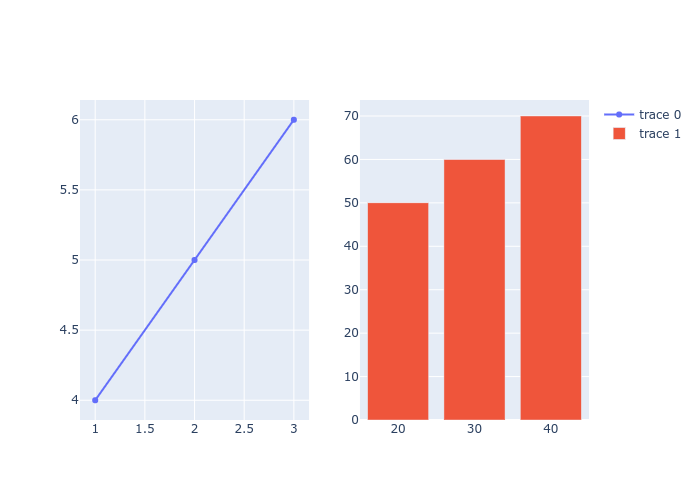
\includegraphics[width=\linewidth]{plot/plotly_two_graph.png}
	\caption{Grafico a dispersione e Istogramma separati}
	\centering
	\label{fig:duePlotDistinti}
\end{figure}
\begin{figure}[h]
	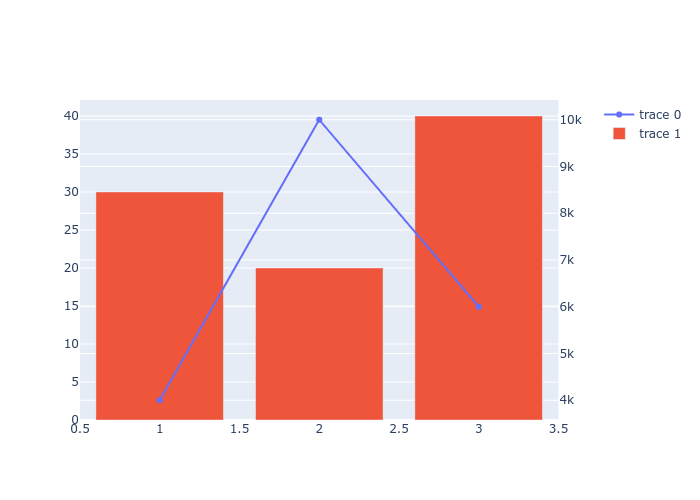
\includegraphics[width=\linewidth]{plot/plot_mixed.png}
	\caption{Grafico a dispersione e Istogramma uniti}
	\centering
	\label{fig:duePlotUniti}
\end{figure}
\clearpage

\section{Il file principale \emph{Main.py}}
Composto  dal omonimo \mintinline{Python}{__name__ == '__main__'} e dalla nuova funzione di 
supporto \mintinline{Python}{entailed_knowledge()}.
\begin{minted}{Python}
def entailed_knowledge():
	patient_sym = read_symptoms(ontology_manager, result=True)
	result = ontology_manager.consistency(condition=True)
	if not result == "The ontology is consistent":
		# Ontologia inconsistente o classi inconsitenti
		print(result)
		ontology_manager.show_classes_iri_my()
		ontology_manager.show_members_in_classes_my()
		# Termina
		sys.exit(5)
	return patient_sym
\end{minted}
In quest'ultima effettua la lettura dei sintomi (vedi \ref{subSec: InputFile}) e salvato il
valore di ritorno si verifica la consistenza della \textbf{KB}. In caso negativo si effettuano delle stampe esplicative e si termina l'esecuzione; altrimenti si ritorna i sintomi, sotto forma di stringa.
                
Il \mintinline{Python}{'__main__'} altro non è che la corretta sequenza di chiamate che 
permette al tool di funzionare: 
\begin{minted}{Python}
if __name__ == '__main__':
	ontology_manager = OntologyManager()
	build_ontology(ontology_manager)
	sym: str = entailed_knowledge()
	IncreasedOntology.compute_probability_for_typical_members(ontology_manager)
	IncreasedOntology.set_probability_for_each_scenario(ontology_manager)
	ontology_manager.show_scenarios()
	query_result = is_logical_consequence(ontology_manager)
	query_result.show_query_result()
	query_result.create_and_show_plot(sym, ontology_manager.cost_dict)
\end{minted}
in primis viene istanziata la classe \mintinline{Python}{OntologyManager}, 
dopodichè viene invocato il metodo \mintinline{Python}{build_ontology} tramite cui viene costruita l'ontologia ed ecco quindi la chiamata all'attività di supporto.
Calcolata le probabilità necessarie per i membri tipici e per gli scenari generati, si passa
alla fase di inferenza e successivamente a quella di analisi dei risultati e generazione dei
grafici. Questo conclude la simulazione.

Abbiamo trattato lo strumento nel modo più completo possibile, cercando, però, di evitare
dettagli o piccolezze trascurabili, focalizzando l'attenzione il più possibile sugli
elementi importanti e peculiari.

                                                            
\begin{comment}

\begin{figure}
\centering
\includegraphics[width=\linewidth]{plot/DepressionEx2.pdf}
\end{figure}
\end{comment}



	
	\chapter{Conclusione e sviluppi futuri}
	Questo breve capitolo finale serve come resoconto di tutto quello
presentato fin’ora e cerca di dare un’idea su come questo tool 
potrebbe essere impiegato, e sulle possibili future evoluzioni che potrà assumere.

Il focus del progetto è il supporto alle decisioni del medico,  l'affiancamento, non la sostituzione di tale figura professionale,

Il considerare i sintomi, normalmente catalogati come atipici, per una certa malattia, 
sotto una diversa luce potrebbe permettere di scoprire che, in realtà, sono indirettamente collegati ad altre patologie.
Per rendere l’idea si pensi ad una persona che soffre di obesità; tendenzialmente 
un obeso ha problemi di metabolismo, scarsa autostima e alti livelli di colesterolo. 
L’utilizzo di smartphone durante i pasti è stato riscontrato essere un fattore incidente sull’aumento di peso, poiché i pazienti testati, tendono a prestare meno attenzione a quello che mangiano e, come conseguenza, ingeriscono maggiori quantità di cibo. 
Questo fatto, indirettamente collegato con l’obesità, potrebbe essere, in alcuni soggetti,
un fattore decisivo. Come conseguenza, questa situazione, se ben rappresentata nella KB, potrebbe esser modellata nello strumento come uno scenario poco probabile, ma sempre possibile; la chiave è avere sottomano lo spettro completo delle alternative.

Per quanto riguarda possibili migliorie, le strade percorribili sono numerose; a partire dall'interfaccia utente: la creazione di una GUI e la semplificazione del processo 
di immissione dati rappresenterebbe un notevole passo avanti per quanto riguarda l'usabilità
e abbasserebbe la curva di apprendimento del software.
Pensando, invece, all'effettivo test ed utilizzo sul campo, è necessario un lavoro di studio,
modifica e creazione di ontologie realistiche o semi-realistiche per dare una parvenza di 
veridicità alle diagnosi prodotte, soprattutto per quanto riguarda le probabilità delle
relazioni e i costi delle diagnosi.
Un altro  possibile percorso potrebbe essere quello di computare e aggiungere ulteriori metadati ai singoli scenari, come, ad esempio, tempistiche indicative e/o un elenco di esami/visite necessarie alla verifica della "diagnosi".
Se dovessimo pensare a delle ottimizzazioni e perfezionamenti, una delle prime idee possibili è l'utilizzodi super-classi \textbf{OWL} più significative del generico \mintinline{XML}{Thing}; classi come
\mintinline{XML}{Patient}, \mintinline{XML}{MedicalIllness} o \mintinline{XML}{Symptom} scritte in un ontologia di supporto.

	
	\appendix
	\chapter{Esempio completo}
	In questa appendice mostreremo un esempio completo di utilizzo di \textit{DbN}, in particolare
l'esempio n.6 dell'articolo \citetitle{ProbOfEx} \cite{ProbOfEx} con la seguente 
$ KB = (\mathcal{T},\mathcal{A}) $

$ \mathcal{T}Box $ :
\begin{itemize}
	\item[] $ Bipolar \sqsubseteq Depressed $
	\item[] $ \mathbf T(Depressed) \sqsubseteq_{0.85} \neg\exists hasSymptom.MoodReactivity $
	\item[] $ \mathbf T(Bipolar) \sqsubseteq_{0.70} \exists hasSymptom.MoodReactivity $
	\item[] $ \mathbf T(ProstateCancerPatient) \sqsubseteq_{0.60} \exists hasSymptom.MoodReactivity $
	\item[] $ \mathbf T(ProstateCancerPatient) \sqsubseteq_{0.80} \exists hasSymptom.Nocturia $
	\item[] $ \mathbf T(Depressed) \sqsubseteq_{0.60} \exists Smart $
\end{itemize}
$\mathcal{A}Box $ :
\[ \{ Depressed(Greg), \neg Smart(Greg) \} \]
Set of \textit{Symptoms} $\mathcal{V} $:
\[ \{ \exists hasSymptom.MoodReactivity(Greg) \} \]
Set of Cost of Disease with \textit{Tipicality}:
\[ \{ Bipolar: 1000, ProstateCancerPatient: 10000, Depressed: 3000 \} \]

Output dello strumento con la seguente ontologia; passo 1, 
verifica della condizione $ KB \cup \mathcal{V} \equiv $ consistente:
\begin{minted}{text}
========== Adding a set of Symptoms to the KB ==========
Sintomo aggiunto: Greg MoodReactivity
========== Checking consistency ==========
========== The ontology is consistent ==========
\end{minted}
passo 2, generazione scenari possibili:
\begin{minted}{text}
INIZIO SCENARIO 1
Typical(Bipolar),Greg,0.7
Probabilità scenario: 0.364
FINE SCENARIO 1

INIZIO SCENARIO 2
Typical(ProstateCancerPatient),Greg,0.48
Probabilità scenario: 0.144
FINE SCENARIO 2

INIZIO SCENARIO 3
Typical(Bipolar),Greg,0.7
Typical(ProstateCancerPatient),Greg,0.48
Probabilità scenario: 0.3356
FINE SCENARIO 3
\end{minted}
passo 3, per ogni scenario si effettua l'inferenza, viene mostrato il primo come esempio:

\begin{minted}{text}
ONTOLOGIA PRIMA DELLA LETTURA DELLA QUERY
Greg member_of Depressed
Greg member_of Not(Smart)
Bipolar is_a [ontoBase.Depressed, owl.Thing]
Depressed is_a [owl.Thing]
MoodReactivity is_a [owl.Thing]
ProstateCancerPatient is_a [owl.Thing]
Nocturia is_a [owl.Thing]
Smart is_a [owl.Thing]
Not(Smart) is_a [owl.Thing]
Not(MoodReactivity) is_a [owl.Thing]
Depressed1 is_a [owl.Thing, ontoBase.r1.only ...
IntersectionDepressedDepressed1 is_a [ontoBase ...
NotDepressed1 is_a [owl.Thing, ontoBase.r1.some( ...
Bipolar1 is_a [owl.Thing, ontoBase.r1.only(Not( ...
IntersectionBipolarBipolar1 is_a [ontoBase ...
NotBipolar1 is_a [owl.Thing, ontoBase.r1.some( ...
ProstateCancerPatient1 is_a [owl.Thing, ontoBase.r1.only ...
IntersectionProstateCancerPatientProstateCancerPatient1 is_a ...
NotProstateCancerPatient1 is_a [owl.Thing, ontoBase.r1.some( ...
FINE ONTOLOGIA PRIMA DELLA LETTURA DELLA QUERY

LETTURA SINTOMI
Sintomo aggiunto: Greg: Not(MoodReactivity)

TRADUCENDO LO SCENARIO: 
INIZIO SCENARIO
Bipolar,Greg,0.7; 
ProbabilitÓ scenario: 0.364
FINE SCENARIO

Membro tipico:
Greg is_a Bipolar
Greg is_a Bipolar1
Greg is_a IntersectionBipolarBipolar1
FINE TRADUZIONE SCENARIO

ONTOLOGIA CON SCENARIO E SINTOMI
Bipolar is_a [ontoBase.Depressed, owl.Thing]
Depressed is_a [owl.Thing]
MoodReactivity is_a [owl.Thing]
ProstateCancerPatient is_a [owl.Thing]
Nocturia is_a [owl.Thing]
Smart is_a [owl.Thing]
Not(Smart) is_a [owl.Thing]
Not(MoodReactivity) is_a [owl.Thing]
Depressed1 is_a [owl.Thing, ontoBase.r1.only ...
IntersectionDepressedDepressed1 is_a [ontoBase ...
NotDepressed1 is_a [owl.Thing, ontoBase.r1.some( ...
Bipolar1 is_a [owl.Thing, ontoBase.r1.only(Not( ...
IntersectionBipolarBipolar1 is_a [ontoBase ...
NotBipolar1 is_a [owl.Thing, ontoBase.r1.some( ...
ProstateCancerPatient1 is_a [owl.Thing, ontoBase.r1.only ...
IntersectionProstateCancerPatientProstateCancerPatient1 is_a ...
NotProstateCancerPatient1 is_a [owl.Thing, ontoBase.r1.some( ...
Greg member_of Depressed
Greg member_of MoodReactivity
Greg member_of Not(Smart)
Greg member_of Not(MoodReactivity)
Greg member_of Bipolar1
Greg member_of IntersectionBipolarBipolar1
FINE ONTOLOGIA CON SCENARIO E SINTOMI
=====================
Il fatto segue logicamente nel seguente scenario: 
INIZIO SCENARIO
Bipolar,Greg,0.7; 
ProbabilitÓ scenario: 0.364
FINE SCENARIO
=====================
ONTOLOGIA PRIMA DELLA LETTURA DELLA QUERY
Greg member_of Depressed
Greg member_of Not(Smart)
Bipolar is_a [ontoBase.Depressed, owl.Thing]
Depressed is_a [owl.Thing]
MoodReactivity is_a [owl.Thing]
ProstateCancerPatient is_a [owl.Thing]
Nocturia is_a [owl.Thing]
Smart is_a [owl.Thing]
Not(Smart) is_a [owl.Thing]
Not(MoodReactivity) is_a [owl.Thing]
Depressed1 is_a [owl.Thing, ontoBase.r1.only ...
IntersectionDepressedDepressed1 is_a [ontoBase ...
NotDepressed1 is_a [owl.Thing, ontoBase.r1.some( ...
Bipolar1 is_a [owl.Thing, ontoBase.r1.only(Not( ...
IntersectionBipolarBipolar1 is_a [ontoBase ...
NotBipolar1 is_a [owl.Thing, ontoBase.r1.some( ...
ProstateCancerPatient1 is_a [owl.Thing, ontoBase.r1.only ...
IntersectionProstateCancerPatientProstateCancerPatient1 is_a ...
NotProstateCancerPatient1 is_a [owl.Thing, ontoBase.r1.some( ...
FINE ONTOLOGIA PRIMA DELLA LETTURA DELLA QUERY

LETTURA SINTOMI
Sintomo aggiunto: Greg: Not(MoodReactivity)

TRADUCENDO LO SCENARIO: 
INIZIO SCENARIO
ProstateCancerPatient,Greg,0.48; 
ProbabilitÓ scenario: 0.14400000000000002
FINE SCENARIO
Membro tipico:
Greg is_a ProstateCancerPatient
Greg is_a ProstateCancerPatient1
Greg is_a IntersectionProstateCancerPatientProstateCancerPatient1

FINE TRADUZIONE SCENARIO
ONTOLOGIA CON SCENARIO E SINTOMI

Bipolar is_a [ontoBase.Depressed, owl.Thing]
Depressed is_a [owl.Thing]
MoodReactivity is_a [owl.Thing]
ProstateCancerPatient is_a [owl.Thing]
Nocturia is_a [owl.Thing]
Smart is_a [owl.Thing]
Not(Smart) is_a [owl.Thing]
Not(MoodReactivity) is_a [owl.Thing]
Depressed1 is_a [owl.Thing, ontoBase.r1.only ...
IntersectionDepressedDepressed1 is_a [ontoBase ...
NotDepressed1 is_a [owl.Thing, ontoBase.r1.some( ...
Bipolar1 is_a [owl.Thing, ontoBase.r1.only(Not( ...
IntersectionBipolarBipolar1 is_a [ontoBase ...
NotBipolar1 is_a [owl.Thing, ontoBase.r1.some( ...
ProstateCancerPatient1 is_a [owl.Thing, ontoBase.r1.only ...
IntersectionProstateCancerPatientProstateCancerPatient1 is_a ...
NotProstateCancerPatient1 is_a [owl.Thing, ontoBase.r1.some( ...
Greg member_of Depressed
Greg member_of MoodReactivity
Greg member_of ProstateCancerPatient
Greg member_of Nocturia
Greg member_of Not(Smart)
Greg member_of Not(MoodReactivity)
Greg member_of ProstateCancerPatient1
Greg member_of IntersectionProstateCancerPatientProstateCancerPatient1

FINE ONTOLOGIA CON SCENARIO E SINTOMI

=====================
Il fatto segue logicamente nel seguente scenario: 
INIZIO SCENARIO
ProstateCancerPatient,Greg,0.48; 
ProbabilitÓ scenario: 0.14400000000000002
FINE SCENARIO
=====================
ONTOLOGIA PRIMA DELLA LETTURA DELLA QUERY

Greg member_of Depressed
Greg member_of Not(Smart)
Bipolar is_a [ontoBase.Depressed, owl.Thing]
Depressed is_a [owl.Thing]
MoodReactivity is_a [owl.Thing]
ProstateCancerPatient is_a [owl.Thing]
Nocturia is_a [owl.Thing]
Smart is_a [owl.Thing]
Not(Smart) is_a [owl.Thing]
Not(MoodReactivity) is_a [owl.Thing]
Depressed1 is_a [owl.Thing, ontoBase.r1.only ...
IntersectionDepressedDepressed1 is_a [ontoBase ...
NotDepressed1 is_a [owl.Thing, ontoBase.r1.some( ...
Bipolar1 is_a [owl.Thing, ontoBase.r1.only(Not( ...
IntersectionBipolarBipolar1 is_a [ontoBase ...
NotBipolar1 is_a [owl.Thing, ontoBase.r1.some( ...
ProstateCancerPatient1 is_a [owl.Thing, ontoBase.r1.only ...
IntersectionProstateCancerPatientProstateCancerPatient1 is_a ...
NotProstateCancerPatient1 is_a [owl.Thing, ontoBase.r1.some( ...
FINE ONTOLOGIA PRIMA DELLA LETTURA DELLA QUERY

LETTURA SINTOMI
Sintomo aggiunto: Greg: Not(MoodReactivity)

TRADUCENDO LO SCENARIO: 
INIZIO SCENARIO
Bipolar,Greg,0.7; ProstateCancerPatient,Greg,0.48; 
ProbabilitÓ scenario: 0.33599999999999997
FINE SCENARIO
Membro tipico:
Greg is_a Bipolar
Greg is_a Bipolar1
Greg is_a IntersectionBipolarBipolar1
Membro tipico:
Greg is_a ProstateCancerPatient
Greg is_a ProstateCancerPatient1
Greg is_a IntersectionProstateCancerPatientProstateCancerPatient1
FINE TRADUZIONE SCENARIO

ONTOLOGIA CON SCENARIO E SINTOMI
Bipolar is_a [ontoBase.Depressed, owl.Thing]
Depressed is_a [owl.Thing]
MoodReactivity is_a [owl.Thing]
ProstateCancerPatient is_a [owl.Thing]
Nocturia is_a [owl.Thing]
Smart is_a [owl.Thing]
Not(Smart) is_a [owl.Thing]
Not(MoodReactivity) is_a [owl.Thing]
Depressed1 is_a [owl.Thing, ontoBase.r1.only ...
IntersectionDepressedDepressed1 is_a [ontoBase ...
NotDepressed1 is_a [owl.Thing, ontoBase.r1.some( ...
Bipolar1 is_a [owl.Thing, ontoBase.r1.only(Not( ...
IntersectionBipolarBipolar1 is_a [ontoBase ...
NotBipolar1 is_a [owl.Thing, ontoBase.r1.some( ...
ProstateCancerPatient1 is_a [owl.Thing, ontoBase.r1.only ...
IntersectionProstateCancerPatientProstateCancerPatient1 is_a ...
NotProstateCancerPatient1 is_a [owl.Thing, ontoBase.r1.some( ...
Greg member_of Depressed
Greg member_of MoodReactivity
Greg member_of ProstateCancerPatient
Greg member_of Nocturia
Greg member_of Not(Smart)
Greg member_of Not(MoodReactivity)
Greg member_of Bipolar1
Greg member_of IntersectionBipolarBipolar1
Greg member_of ProstateCancerPatient1
Greg member_of IntersectionProstateCancerPatientProstateCancerPatient1
FINE ONTOLOGIA CON SCENARIO E SINTOMI

Il fatto segue logicamente nel seguente scenario: 
INIZIO SCENARIO
Bipolar,Greg,0.7; ProstateCancerPatient,Greg,0.48; 
ProbabilitÓ scenario: 0.33599999999999997
FINE SCENARIO
\end{minted}

\clearpage

passo 4, elenco degli scenari verificati e relativo grafico:
\begin{minted}{text}
RISULTATI DELL'INTERROGAZIONE: 
SCENARI IN CUI LA QUERY SEGUE LOGICAMENTE
INIZIO SCENARIO 1
Bipolar,Greg,0.7; 
Probabilità complessiva dello scenario: 0.364
FINE SCENARIO 1

INIZIO SCENARIO 2
ProstateCancerPatient,Greg,0.48; 
Probabilità complessiva dello scenario: 0.14400000000000002
FINE SCENARIO 2

INIZIO SCENARIO 3
Bipolar,Greg,0.7; ProstateCancerPatient,Greg,0.48; 
Probabilità complessiva dello scenario: 0.33599999999999997
FINE SCENARIO 3

PROBABILITÀ TOTALE: 0.844

Fine simulazione, tempo totale:  1.984983205795288  s
\end{minted}

\paragraph{Analisi dei risultati} \hfill

Possiamo vedere nelle figure \ref{fig: A_web} ed \ref{fig: A_doc} una rappresentazione
grafica dei risultati finali. Iniziamo dunque descrivendo i tre assi cartesiani (due x e uno y) e il loro significato magari non immediato. L'asse x 
contiene il numero della diagnosi (1,2,3) con il suo corrispettivo istogramma e 
punto della funzione a dispersione, infatti ,sui due assi y, troviamo raffigurata sia la probabilità della diagnosi (scenario) $ t $, 
espressa in percentuale `\%`, sia il costo stimato della stessa,
espressa in €. Come rappresentazione si è scelto nel primo caso un istogramma al
cui interno troviamo
la/le malattia/e considerata/e come possibile spiegazione. 
Ogni rettangolo è identificato con colore diverso per la variabile, per darne risalto, essendo
un fattore importante che facilità la scelta 
dell'eventuale iter terapeutico. Per quanto riguarda la spesa medica si è preferito un
grafico a dispersione in quanto questo criterio decisionale è secondario alla salute del 
paziente e, soprattutto necessita ulteriori sviluppi.

In conclusione si fa notare al lettore la presenza della legenda riassuntiva e delle etichette esplicative sui relativi assi,
in particolare la probabilità complessiva delle possibili diagnosi (escluso lo scenario vuoto, cioè nessuna spiegazione).

\begin{figure}
	\centering
	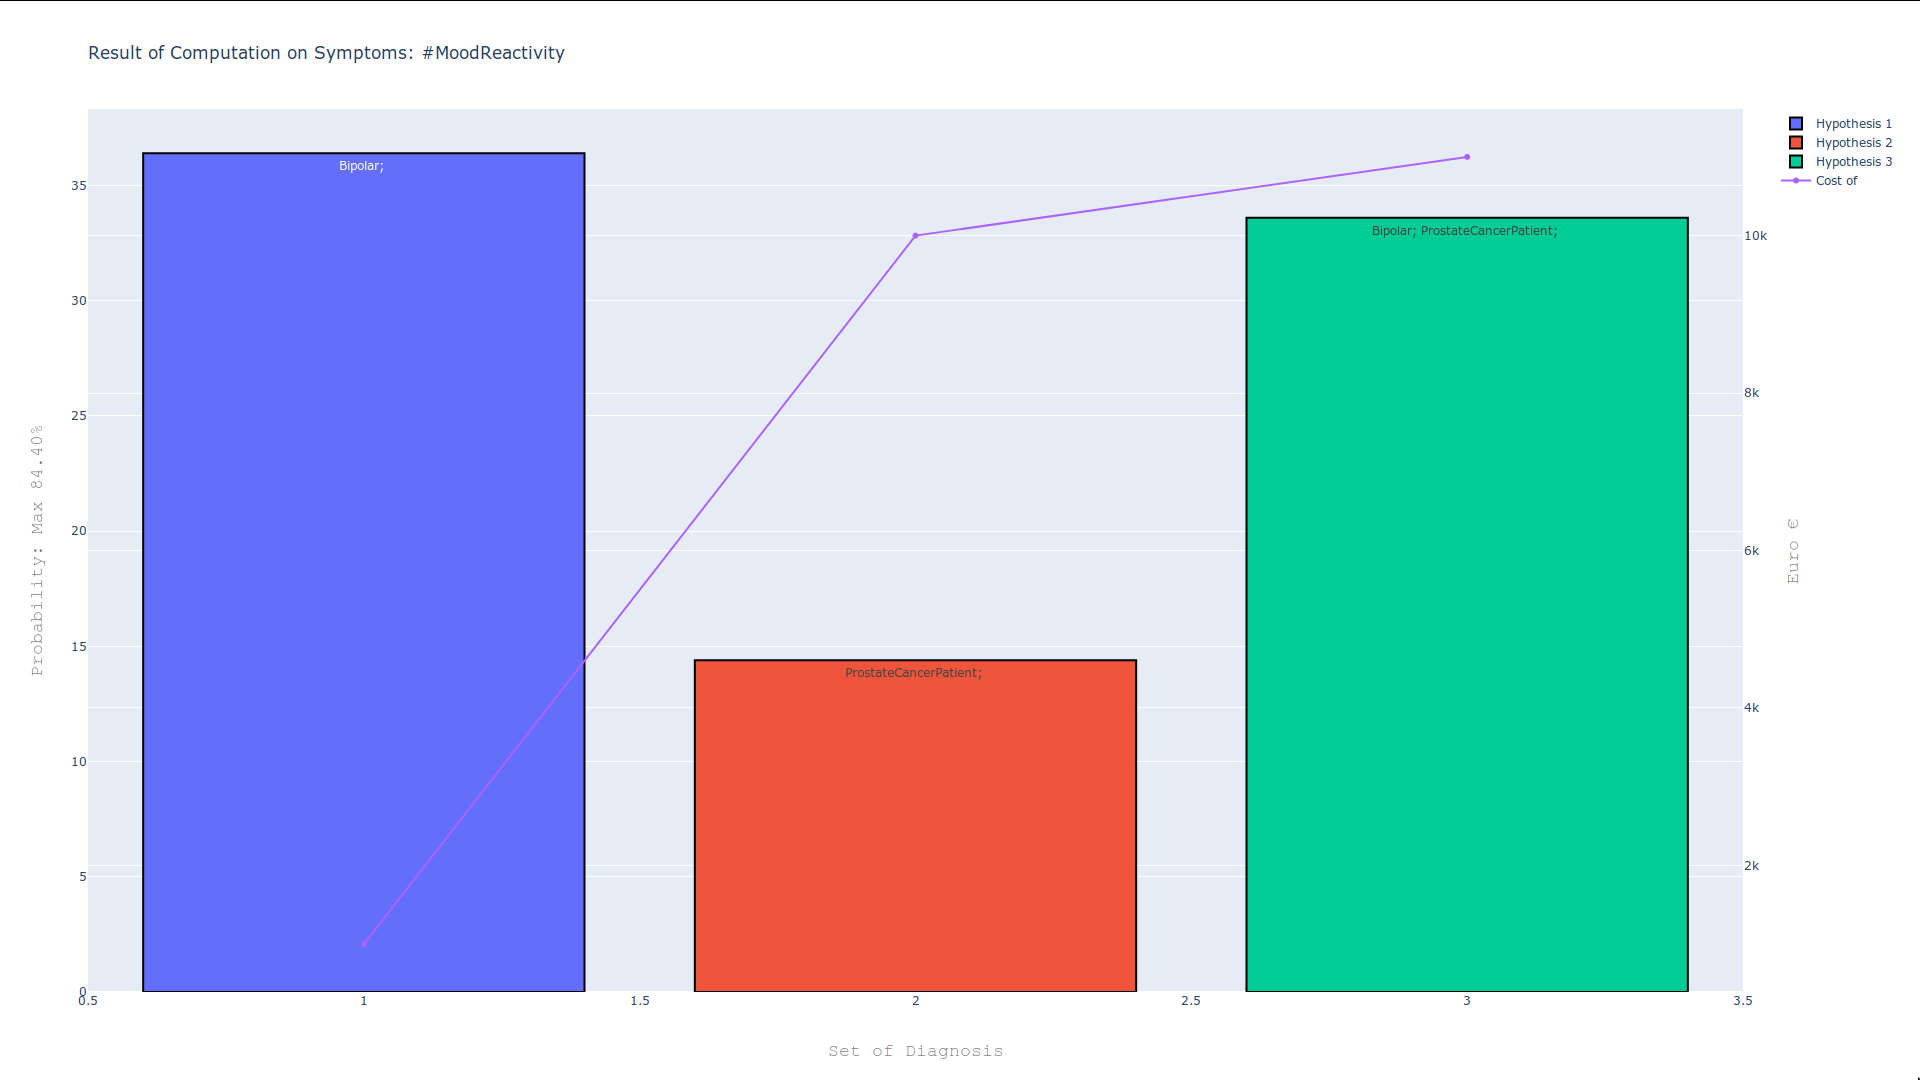
\includegraphics[width=\linewidth]{plot/Caso_di_studio.png}
	\caption{Versione Web}
	\label{fig: A_web}
\end{figure}

\begin{figure}
	\centering
	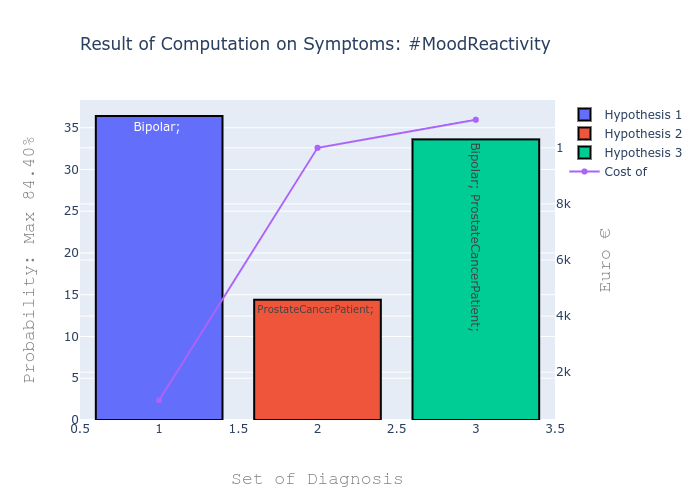
\includegraphics[width=\linewidth]{plot/caso_di_studio_alt.png}
	\caption{Versione documento}
	\label{fig: A_doc}
\end{figure}
	
	\printbibliography
	
		
	%\chapter*{Dedication}
	%To mum and dad
	
	%\chapter*{Declaration}
	%I declare that..
	
	%\chapter*{Acknowledgements}
	%I want to thank...
	
\end{document}